\documentclass[twoside,a4paper,11pt,addpoints]{exam}%answers,answers



\title{XX 1}
\date{}
\author{Juliette Fenogli}


\usepackage{siunitx}
\usepackage{mystyles}
\usepackage[export]{adjustbox}
\usepackage{mathpazo}
\usepackage{booktabs}
\usepackage{framed}
\usepackage{mdframed}
\usepackage[most]{tcolorbox}
\usepackage{listings}
\usepackage{mhchem}
\usepackage{tcolorbox}

\usepackage{subfig}
\usepackage{float}

\lstset
{upquote=true,
columns=flexible,
    basicstyle=\small\tt\hbox{}, 
	basicstyle=\ttfamily,
	language=Python,
    framesep=\fboxsep,
    framerule=\fboxrule,
    xleftmargin=\dimexpr\fboxsep+\fboxrule,
    xrightmargin=\dimexpr\fboxsep+\fboxrule,
	commentstyle=\color{gray},
	frame=single,
	rulecolor=\color{green!5},
	backgroundcolor=\color{gray!5},
	breaklines,
	numbers=left, 
	numbersep=5pt,  
	numberstyle=\scriptsize \ttfamily\color{gray},
	breakindent=1.5em,
	literate={Δ}{{$\mathtt{\Delta}$}}1 {‡}{{$\mathtt{\ddagger}$}}1
  {á}{{\'a}}1 {é}{{\'e}}1 {í}{{\'i}}1 {ó}{{\'o}}1 {ú}{{\'u}}1
  {Á}{{\'A}}1 {É}{{\'E}}1 {Í}{{\'I}}1 {Ó}{{\'O}}1 {Ú}{{\'U}}1
  {à}{{\`a~}}1 {è}{{\`e}}1 {ì}{{\`i}}1 {ò}{{\`o}}1 {ù}{{\`u}}1
  {À}{{\`A~}}1 {È}{{\'E}}1 {Ì}{{\`I}}1 {Ò}{{\`O}}1 {Ù}{{\`U}}1
  {ä}{{\"a}}1 {ë}{{\"e}}1 {ï}{{\"i}}1 {ö}{{\"o}}1 {ü}{{\"u}}1
  {Ä}{{\"A}}1 {Ë}{{\"E}}1 {Ï}{{\"I}}1 {Ö}{{\"O}}1 {Ü}{{\"U}}1
  {â}{{\^a}}1 {ê}{{\^e}}1 {î}{{\^i}}1 {ô}{{\^o}}1 {û}{{\^u}}1
  {Â}{{\^A}}1 {Ê}{{\^E}}1 {Î}{{\^I}}1 {Ô}{{\^O}}1 {Û}{{\^U}}1
  {œ}{{\oe}}1 {Œ}{{\OE}}1 {æ}{{\ae}}1 {Æ}{{\AE}}1 {ß}{{\ss}}1
  {ç}{{\c c}}1 {Ç}{{\c C}}1 {ø}{{\o}}1 {å}{{\r a}}1 {Å}{{\r A}}1
  {€}{{\EUR}}1 {£}{{\pounds}}1 {×}{{$\times$}}1,       
}


\usepackage{adjustbox}
\usepackage{colortbl}
\usepackage{fontawesome}
\usepackage{todonotes}
\usepackage{listings} %codes python
\usepackage{parskip}

%Columns Spacing
\newcolumntype{C}[1]{>{\centering\let\newline\\\arraybackslash\hspace{0pt}}m{#1}}
\newcolumntype{M}[1]{>{\centering\arraybackslash}m{#1}}

%Colorbox
\newtcolorbox{mybox}{colback=white!5!white,
colframe=black!75!black,left=7mm}

\newcounter{foo} %Counter questions

\begin{document}

\begin{minipage}{0.33\textwidth}
Noms-Prénoms du binôme
\end{minipage}\begin{minipage}{0.33\textwidth}
$n^\circ 1$ :
\end{minipage}\begin{minipage}{0.33\textwidth}
$n^\circ 2$ :
\end{minipage}



\tito{Expériences autour des concepts de base d'électrochimie pour l'énergie}

\paragraph*{But} 
Lors de cette séance de TP, vous serez emmené à revisiter les concepts élémentaires des réactions redox par une approche expérimentale. Avant toute chose, l'objectif est de se familiariser avec plusieurs concepts théoriques vus dans les deux premiers chapitres du cours sur les batteries.

\paragraph*{Quelques remarques :}
\begin{enumerate}
\item Votre présence physique en travaux pratique doit s'accompagner d'une connaissance des notions du cours $n^\circ 1$ et $2$.
\item La lecture des annexes du TP doit avoir préalablement faites doit avoir été fait en amont.
\item Toute figure doit comporter des axes, des unités, un titre et des légendes. Le titre doit permettre à l'enseignant de comprendre l'essentiel de la figure sans avoir à lire le texte associé.
\item Toute donnée expérimentale doit être accompagnée des conditions expérimentales et des outils de mesure utilisés.
\item Toutes les mesures devront être accompagnées d'un nombre cohérent de chiffres significatifs et d'unités.%Les incertitudes de type B devront être évaluées dans tous les outils de mesure utilisés (voltmètre, ampèremètre, thermomètre$\ldots$ à l'aide de fiches fournies en début de TP.
\item Les questions en {\color{purple} violet} doivent avoir été réfléchies en amont du TP. En l'absence de recherche de votre part, l'enseignant en charge du TP sanctionnera le groupe.
\end{enumerate}

\tableofcontents

\section{\'{E}chelle de potentiel électrochimique - \faClockO ~ \SI{30}{\minute}}

Vous cherchez à mettre en place une pile galvanique présentant les meilleures performances énergétiques. Pour cela, vous allez devoir classer des métaux en fonction de leur noblesse, notion expérimentale. Par définition, un métal est dit noble lorsqu'il résiste à la corrosion et à l'oxydation.

Lors de votre arrivée au laboratoire, votre travail sera contraint par le matériel disponible :
\begin{center}
\begin{tabular}{ccc}
Solides & Solutions à \SI{0.01}{\mole\per\liter} & Verrerie \\
\ce{Cu(s)} & \ce{Cu^{2+} (aq)} & Pipette Pasteur \\
\ce{Zn(s)} & \ce{Zn^{2+} (aq)} & \\
\ce{Al (s)} & \ce{Al^{3+} (aq)} & \\
\ce{Ag (s)} & \ce{Ag^+ (aq)} & \\
\ce{Fe (s)} & \ce{Fe^{2+} (aq)} &
\end{tabular}
\end{center}

\faWarning ~ Vous veillerez lors de vos tests à bien vérifier l'état de surface de vos électrodes. Sinon, il faudra envisager de les poncer en surface ou de les passer quelques secondes à l'acide nitrique concentré (attention, manipulation sous hôte et gant avec aération).

\begin{questions}

%\begin{tcolorbox}[breakable, enhanced, color=white]
\begin{mybox}
\question[3] \label{Q:01} {\color{purple} Proposer une démarche d'investigation permettant de classer ces métaux en fonction de leur noblesse.}
\begin{solution}[8cm]

Les étudiants sont emmenés à réaliser des tests qualitatifs en déposant une goutte de solution sur chacune des plaques métalliques (le dépôt de la solution contenant le contre-ion du métal est sans intérêt). En cas d'apparition d'un dépôt métallique au niveau de la goutte, l'étudiant conclut que le métal de la plaque a réagi avec l'ion présent en solution.

\begin{center}

\includegraphics[width=8cm]{figures/Corr01}
\end{center}


La démarche d'investigation doit conduire les étudiants à réaliser un tableau à deux entrées : 

\begin{center}
\begin{tabular}{|c|c|c|c|c|c|}
\hline
Solution déposée / Solide & \ce{Ag (s)} & \ce{Cu(s)} & \ce{Fe (s)} & \ce{Zn (s)} & \ce{Al (s)} \\
\hline
\ce{Ag^+ (aq)} & \cellcolor{gray} & \cellcolor{green} & \cellcolor{green} & \cellcolor{green} & \cellcolor{green} \\
\hline
\ce{Cu^{2+} (aq)} & \cellcolor{red} & \cellcolor{gray} & \cellcolor{green} & \cellcolor{green} & \cellcolor{green} \\
\hline
\ce{Fe^{2+} (aq)} & \cellcolor{red} & \cellcolor{red} & \cellcolor{gray} & \cellcolor{green} & \cellcolor{green} \\
\hline
\ce{Zn^{2+} (aq)} & \cellcolor{red} & \cellcolor{red} & \cellcolor{red} & \cellcolor{gray} & \cellcolor{green} \\
\hline
\ce{Al^{3+} (aq)} & \cellcolor{red} & \cellcolor{red} & \cellcolor{red} & \cellcolor{red} & \cellcolor{gray} \\
\hline
\end{tabular}
\captionof{table}{Tableau à deux entrées permettant de classer les métaux en fonction de leur inertie chimique [$\color{green} \blacksquare$ apparition d'un dépôt; $\color{red} \blacksquare$ absence de dépôt]}

Au bilan, on peut classer les métaux du plus noble au moins noble dans cette série :
\begin{align}
\ce{Ag} > \ce{Cu} > \ce{Fe} > \ce{Zn} > \ce{Al}  
\end{align}
\end{center}

avec ">" qui signifie \og plus noble que \fg{}

\end{solution}
\end{mybox}
%\end{tcolorbox}

\begin{mybox}
\question[1] \label{Q:02} Déduire de la Q. \ref{Q:01}, l'ordre attendu des potentiels standard des couples mis en jeu à température ambiante.

\begin{solution}[3cm]
Les étudiants doivent associer la "noblesse" de l'espèce à sa capacité à oxyder. Or ils savent que le meilleur oxydant présente le potentiel redox le plus élevé.
\begin{align*}
E^\circ (\ce{Ag+ / Ag} ) > E^\circ (\ce{Cu^{2+} / Cu} ) > E^\circ (\ce{Fe^{2+} / Fe} ) > E^\circ (\ce{Zn^{2+} / Zn} ) > E^\circ (\ce{Al^{3+} / Al} )
\end{align*}

Ces valeurs peuvent être mises en relief avec les données de la littérature à \SI{298}{\kelvin}.

\begin{center}
\begin{tabular}{cccccc}
Couple & \ce{Ag+ / Ag} & \ce{Cu^{2+} / Cu} & \ce{Fe^{2+} / Fe} & \ce{Zn^{2+} / Zn} & \ce{Al^{3+} / Al} \\
$E^\circ $ & 0.80 & 0.34 & -0.44 & -0.76 & -1.66 \\
\end{tabular}
\captionof{table}{Potentiel redox standard des couples à \SI{298}{\kelvin}}
\end{center}
%E°
%Al3+/Al -1.66
%Zn2+/Zn −0,7618
%Cu2+/Cu +0,340
%Ag+/Ag +0,7996
%Fe2+/Fe  −0,44
\end{solution}
\end{mybox}

\begin{mybox}
\question[1] \label{Q:03} Rappeler ce qu'est la qualité de l'énergie. Si on souhaite disposer de la cellule électrochimique avec la meilleure qualité d'énergie, quels couples en théorie devrions-nous choisir ?

\begin{solution}[5cm]
Les étudiants ont vu la modélisation Thévenin d'une pile, modèle critiqué dans la suite du sujet. 

\begin{center}
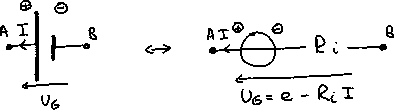
\includegraphics[width=0.5\textwidth]{figures/Corr05}
\end{center}

Ils savent que la puissance émise par la pile est donnée par :
\begin{align*}
P = e \cdot I - R \cdot I^2
\end{align*}
où $e$ est la f.e.m., $R$ est la résistance interne.

Afin de minimiser le terme associé à l'effet Joule/chute ohmique, les étudiants doivent proposer le couple redox maximisant la f.e.m. : 
\begin{align*}
e &\approx e^\circ \approx  E^\circ_\oplus - E^\circ_\ominus \\
&\approx E^\circ ( \ce{Ag+ / Ag} ) - E^\circ ( \ce{Al^{3+} / Al} ) \\
&\stackrel{AN}{=} 2.42 ~ \si{\volt}
\end{align*}
Le couple \ce{Ag+ / Ag} et \ce{Al^{3+} / Al} présentent la meilleure qualité d'énergie en théorie.
\end{solution}
\end{mybox}

L'aluminium est un métal qui a tendance à se passiver naturellement au contact de l'eau. Afin de comprendre ce qu'il peut se passer, on se propose d'étudier le diagramme de Pourbaix (E-pH) de cet élément au contact d'un milieu aqueux : 

\begin{center}
\begin{minipage}{0.58\textwidth}

\includegraphics[width=\textwidth]{figures/Fig04}
\end{minipage}\begin{minipage}{0.38\textwidth}
\captionof{figure}{Diagramme E-pH de l'aluminium et de l'eau à \SI{25}{\celsius} [la convention de tracé est fixée à \SI{1}{\mole\per\liter}]}
\label{fig:04}
\end{minipage}
\end{center}

\begin{mybox}
\question[1] \label{Q:04} Définir le terme \og passivation naturelle \fg{}. En vous appuyant sur la Fig. \ref{fig:04}, argumenter la nature chimique de la couche de passivation. Faites un schéma d'une plaque d'aluminium et représenter la couche de passivation. En quoi est-ce un souci pour la réalisation d'une pile ?

\begin{solution}[6cm]
Protection d'un métal ou d'un alliage métallique contre la corrosion grâce à la formation d'une couche d'oxyde protectrice.\\

Dans le cas de l'aluminium, la passivation s'obtient naturellement au contact de l'eau ou de l'air.\\

Le diagramme de Pourbaix (E-pH) nous renseigne sur les domaines de stabilité thermodynamique de l'aluminium, oxyde et hydroxyde au contact de l'eau (corrosion humide). \`{A} pH autour de 7, on observe que l'aluminium se corrode au contact de l'eau, sous forme d'hydroxydes d'aluminium ou d'oxydes d'aluminium, communément appelé alumine. 

Un schéma analogue au suivant peut être proposé : 
\begin{center}
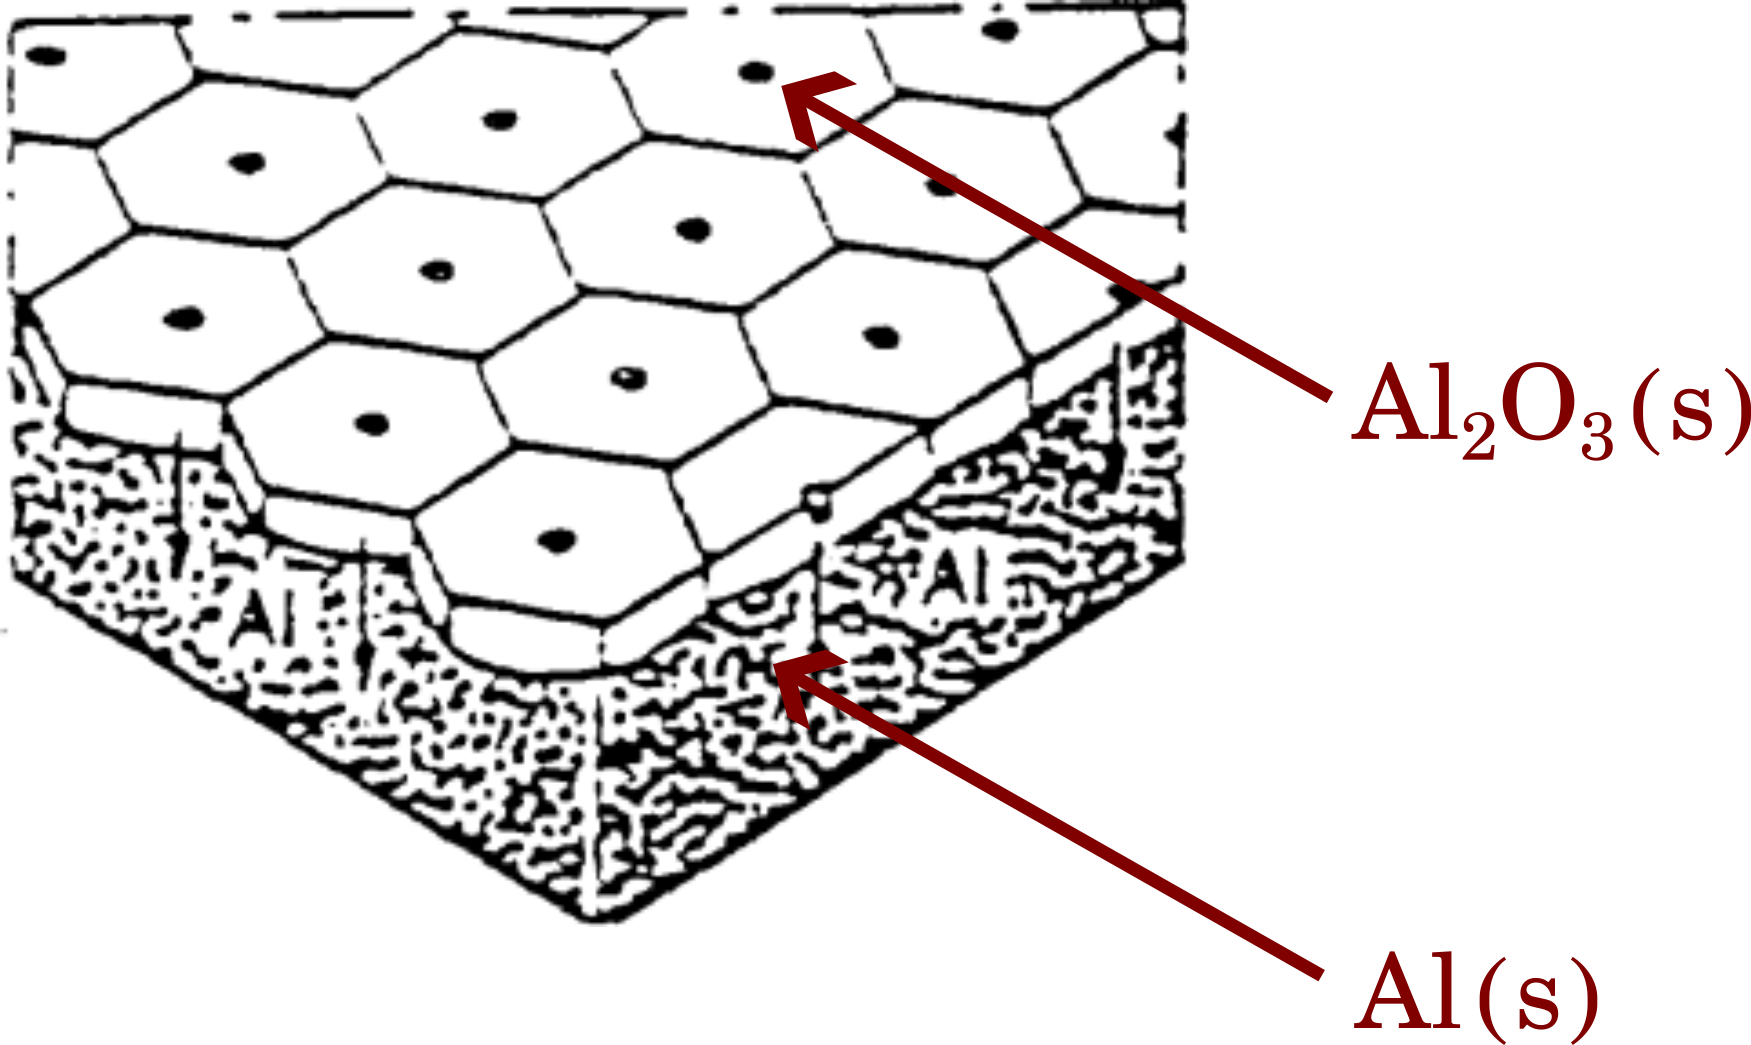
\includegraphics[height=3cm]{figures/Corr04}
\end{center}%Vigne, Une vie d'aluminium

L'apparition de l'alumine pose deux soucis techniques :
\begin{enumerate}
\item l'aluminium n'est plus en contact avec les ions aluminium (isolant ionique) ;
\item l'aluminium ne permet pas le passage des électrons (isolant électronique) vers le circuit électrique.
\end{enumerate}

\end{solution}
\end{mybox}

Du fait des contraintes matérielles, dans la suite du sujet, nous nous limiterons à l'utilisation des couples \ce{Zn^{2+} (aq)}/\ce{Zn (s)} et \ce{Cu^{2+} (aq)}/\ce{Cu (s)}.

\setcounter{foo}{\value{question}}
\end{questions}

\paragraph*{Données} 
\begin{itemize}
\item Potentiel standard en \si{\volt\per{ESH}} à \SI{298}{\kelvin} :
\begin{center}
\begin{tabular}{cccccc}
\toprule
Couple & \ce{Ag+ / Ag} & \ce{Cu^{2+} / Cu} & \ce{Fe^{2+} / Fe} & \ce{Zn^{2+} / Zn} & \ce{Al^{3+} / Al} \\
\midrule
$E^\circ $ & 0.80 & 0.34 & -0.44 & -0.76 & -1.66 \\
\bottomrule
\end{tabular}
\end{center}

\item Résistivité électrique de quelques matériaux à \SI{293}{\kelvin} :
\begin{center}
\begin{tabular}{cccccc}
\toprule
Couple & Al & \ce{Al2O3} \\
\midrule
$\rho ~ [\si{\ohm\meter}] $ & $10^{-3}$ & $10^{12}$ \\
\bottomrule
\end{tabular}
\end{center}
\end{itemize}

%Cette section comporte {\thefoo} questions pour un total de {\numpoints} points sur 20.

\newpage

\section{Détermination de grandeurs thermodynamique et cinétique de cellules électrochimiques}

\subsection{Mesure de la force électromotrice - \faClockO ~ \SI{30}{\minute}}

\paragraph*{Schéma du montage}
\begin{center}
\begin{minipage}{0.48\textwidth}

\includegraphics[width=\textwidth]{figures/Fig01}
\end{minipage}\begin{minipage}{0.48\textwidth}
\captionof{figure}{Montage expérimental permettant la mesure de la force électromotrice.}
\label{fig:01}
\end{minipage}
\end{center}

\paragraph*{Protocole expérimental}
\begin{enumerate}
\item Prendre deux béchers thermostatés de \SI{400}{\milli\liter}, les recouvrir de papier aluminium à l'extérieur afin de limiter les déperditions thermiques ;
\item Connecter en circuit fermé ces deux béchers au bain thermostaté, puis allumer la circulation d'eau ;
\item Régler le bain à \SI{20}{\celsius} ;
\item Verser \SI{100}{\milli\liter} d'une solution de sulfate de zinc et une solution de sulfate de cuivre dans chacun des béchers ;
\item Ajouter quelques gouttes d'acide sulfurique concentré et vérifier le pH ($\approx 4-5$);
\item Installer les électrodes, les connectiques, le pont salin contenant du nitrate d'ammonium \ce{NH4NO3} gélifié et le thermomètre dans un des béchers ;
\item Installer le voltmètre.
\end{enumerate}

\hspace{0.5cm}

\begin{questions}
\setcounter{question}{\thefoo}
\begin{mybox}
\question[1] Représenter en notation simplifiée le montage chimique de la pile.

\begin{solution}[2cm]
On indique par $|$ les interfaces et par $\ominus/\oplus$ les pôles à l'aide de l'étude de corrosion de la partie précédente.

\begin{equation*}
\ominus ~ \ce{Zn (s)} | \ce{Zn^{2+} (aq)} ; \ce{SO_4^{2-} (aq)} | \ce{K^+ (aq)} ; \ce{NO_3^{2-} (aq)} | \ce{Cu^{2+} (aq)} ; \ce{SO_4^{2-} (aq)} | \ce{Cu (s)} ~ \oplus
\end{equation*}
\end{solution}
\end{mybox}

\begin{mybox}
\question[1] \`{A} l'aide du voltmètre, vérifier la polarité de la pile et relever la tension à courant nul. Schématiser les deux situations puis compléter la question précédente en indiquant les pôles.

\begin{solution}[5cm]

\begin{figure}[H]
\begin{center}
\subfloat[\label{fig:Corr02a}]{
\includegraphics[width=3cm]{figures/Corr02a}}\hspace{1cm}\subfloat[\label{fig:Corr02b}]{
\includegraphics[width=3cm]{figures/Corr02b}}
\caption{\ref{fig:Corr02a} Circuit équivalent permettant d'obtenir une tension positive ; \ref{fig:Corr02b} Circuit équivalent permettant d'obtenir une tension négative.}
\end{center}
\end{figure}

Les étudiants trouvent autour de \SI{1.1}{\volt}.


En changeant l'orientation du voltmètre, les étudiants remarquent que la tension indiquée est positive (voir Fig. \ref{fig:Corr02a}) ou négative (voir \ref{fig:Corr02b}), ils peuvent confirmer la polarité de la pile.
\end{solution}
\end{mybox}

\begin{mybox}
\question[1] Compléter le schéma de /la Fig.\ref{fig:01}, lorsque la pile se décharge en indiquant : la polarité, le sens du courant et de circulation des électrons ainsi que l'anode et la cathode. Donner les demi-équations redox associé à chaque demi-pile.
\begin{solution}[5cm]
\begin{center}

\includegraphics[width=8cm]{figures/Corr03}
\begin{minipage}{0.48\textwidth}
\begin{align*}
\ce{Zn (s, \ominus) = Zn^{2+} (aq, \ominus) + 2e^-}
\end{align*}
\end{minipage}\begin{minipage}{0.48\textwidth}
\begin{align*}
\ce{Cu^{2+} (aq, \oplus) + 2e^- = Cu(s, \oplus)}
\end{align*}
\end{minipage}\end{center}
\end{solution}

\end{mybox}

\begin{mybox}
\question[\half] En déduire l'équation de réaction fictive associée à cette pile.
\begin{solution}[2cm]
\begin{center}
\begin{minipage}{0.4\textwidth}
\begin{align*}
\ce{Zn (s, \ominus) + Cu^{2+} (aq, \oplus) =  Zn^{2+} (aq, \ominus) + Cu(s, \oplus)}
\end{align*}
\end{minipage}
\end{center}

\end{solution}
\end{mybox}
\setcounter{foo}{\value{question}}
\end{questions}

\newpage

\subsection{Caractéristique et interprétation  - \faClockO ~ \SI{3}{\hour}}

\subsubsection{Tracé de la caractéristique et confrontation au modèle linéaire}

Une modélisation commune de la caractéristique électrique d'une pile consiste à assimiler la pile à un \textbf{dipôle linéaire} résultant de l'association d'un générateur de tension de force électromotrice $e$ et d'une résistance de résistance $R$.

\begin{figure}[H]
\begin{minipage}{0.48\textwidth}

\includegraphics[width=\textwidth]{figures/Fig06}
\end{minipage}\hfill\begin{minipage}{0.48\textwidth}
\caption{Modélisation de la pile comme un dipôle linéaire résultant de l'association en série d'un générateur de tension et d'une résistance interne.}
\label{fig:06}
\end{minipage}
\end{figure}

Dans un tel modèle, la tension de la pile devrait s'écrire comme : 
\begin{align*}
U_G = e - R \cdot I
\end{align*}

La force électromotrice, notée $e$, est la tension prédite par la thermodynamique, tandis que la résistance interne, notée $R$, prend en compte les phénomènes dissipatifs associés à la migration des ions (dans les solutions et le pont salin) ou des électrons (dans les plaques). 

Nous allons chercher à discuter la validité et les limites de ce modèle.


\paragraph*{Schéma du montage}

Pour comprendre les différents effets thermodynamique et cinétique ayant lieu dans la pile, on se propose de construire les deux montages ci-dessous :

\begin{center}
\begin{minipage}{0.48\textwidth}

\includegraphics[width=0.95\textwidth]{figures/Fig07a}
\end{minipage}\begin{minipage}{0.48\textwidth}

\includegraphics[width=0.95\textwidth]{figures/Fig07b}
\end{minipage}
\captionof{figure}{Montages à réaliser pendant les travaux pratiques avec dans la partie électrique : un ampèremètre, trois voltmètres et un générateur de tension, de tension $U_G$. Le courant $I$ indique le courant sortant de la pile.}
\label{fig:07}
\end{center}

Le montage de gauche permet de faire l'acquisition de la caractéristique pour une tension globale de la pile positive, tandis que le montage de droite le permet pour une tension globale de la pile négative.

On rappelle que l'électrode au calomel saturée, notée ECS, est une électrode dont le potentiel est constant par rapport à l'ESH.




\paragraph*{Matériel à votre disposition}

%En plus du matériel indiqué à la Fig. \ref{fig:07}, on met à votre disposition le matériel suivant : 
%\begin{itemize}
%\item quatre multimètres ;
%\item des fils ; 
%\item deux électrodes au calomel saturée ;
%\end{itemize}

%\hspace{0.5cm}

% Placer dans le dispositif expérimental de la Fig. \ref{fig:07}, les électrodes de référence et les voltmètre pour mesurer : le potentiel d'électrode $\oplus$, le potentiel d'électrode $\ominus$ et l'ensemble (potentiel de jonction + tension de résistance dans la pile). Ajouter ensuite le dernier ampèremètre afin de faire l'acquisition du courant, de telle sorte que la \textbf{pile Daniell soit en convention générateur}. Un ou des schémas expérimentaux sont attendus.
\begin{questions}
\setcounter{question}{\thefoo}
\begin{mybox}
\question[1] {\color{purple} Indiquer ce que l'on mesure à chacun des voltmètre et ampèremètre.}
\begin{solution}[8cm]
On a dans les deux situations le courant $I$ qui est le courant sortant de la pile et trois tensions qui sont mesurées : $U_\oplus$, $U$ et $U_\ominus$.

\begin{center}
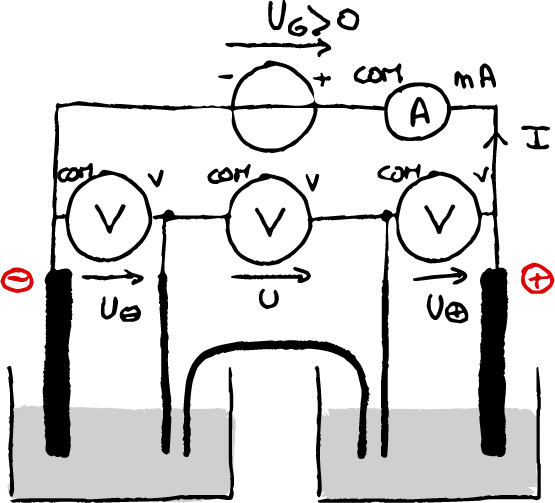
\includegraphics[width=0.48\textwidth]{figures/Corr06a}\hfill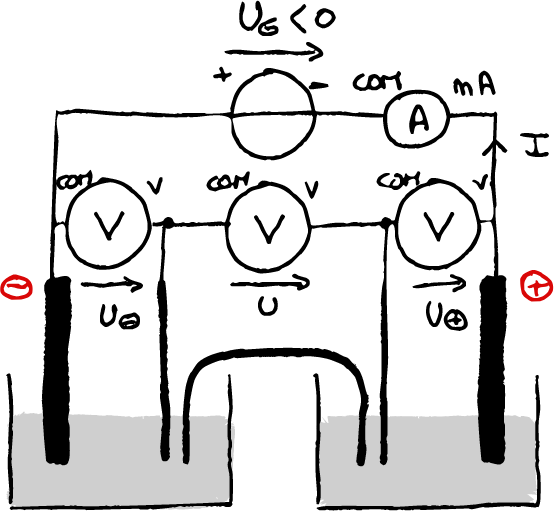
\includegraphics[width=0.48\textwidth]{figures/Corr06b}
\captionof{figure}{Le montage à gauche permet la mesure des tensions positives de la pile, le montage de droite des tensions négatives de la pile}
\end{center}

Dans ces deux situations, les tensions mesurent : 
\begin{itemize}
\item[$U_\oplus$] le potentiel de l'électrode $\oplus$ par rapport à l'ECS ;
\item[$U$] la potentiel du compartiment $\oplus$ par rapport au compartiment $\ominus$, qui sera associée à la résistance de la solution ;
\item[$U_\ominus$] le potentiel de l'électrode $\ominus$ par rapport à l'ECS.
\end{itemize}

\end{solution}
\end{mybox}

%\question[1] Appeler l'enseignement pour qu'il vérifie le montage électrique et chimique.

\begin{mybox}
\question[2] {\color{purple} Décomposer le potentiel électrostatique, noté $\Phi$, entre la borne $\oplus$ et $\ominus$ de la pile, et démontrer que l'on fait bien l'acquisition des tensions indiquées à la question précédente. On pourra exprimer cela sous la forme : 
\begin{align*}
U_G [V] &= E_\oplus [V/ECS] + U [V] - E_\ominus [V/ECS]
\end{align*}
avec $E_\oplus$ le potentiel de l'électrode $\oplus$ par rapport à l'ECS, $E_\ominus$ le potentiel de l'électrode $\ominus$ par rapport à l'ECS et $U$ la chute ohmique dans la pile.
}\\ 
\emph{Aide : Pour cela, vous aurez besoin de faire apparaître le potentiel électrostatique aux électrodes $\oplus$ \& $\ominus$, le potentiel électrostatique à chacune des électrodes au calomel saturé et le potentiel électrostatique au sein de la solution dans chacun des compartiments.}
\begin{solution}[8cm]
On peut décomposer le potentiel électrostatique : 
\begin{align*}
U_G &= \Phi_\oplus - \Phi_\ominus \\
&= \underbrace{(\Phi_\oplus - \Phi_{S_\oplus})}_{E_\oplus} + \underbrace{(\Phi_{S_\oplus} - \Phi_{ECS_\oplus})}_{-E_{ECS,\oplus}} + \underbrace{(\Phi_{ECS_\oplus} - \Phi_{ECS_\ominus})}_{U} - \underbrace{(\Phi_{S_\ominus} - \Phi_{ECS_\ominus})}_{-E_{ECS,\ominus}} - \underbrace{(\Phi_{\ominus} - \Phi_{S_\ominus})}_{E_\ominus} \\
&= (E_\oplus [\si{\volt\per{ESH}}] - E_{ECS, \oplus} [\si{\volt\per{ESH}}]) + U - (E_\ominus [\si{\volt\per{ESH}}] - E_{ECS, \ominus} [\si{\volt\per{ESH}}]) \\
U_G &= E_\oplus [\si{\volt\per{ECS}}] + U - E_\ominus [\si{\volt\per{ECS}}]
\end{align*}
Lors de la mesure, on a trois tensions : 
\begin{itemize}
\item la tension $U_\oplus$ assimilable au potentiel à la $E_\oplus$ par rapport à l'ECS ;
\item la tension $U$ assimilable à la chute ohmique ;
\item la tension $U_\ominus$ assimilable à l'inverse du potentiel $E_\ominus$ par rapport à l'ECS.
\end{itemize}

\end{solution}
\end{mybox}

Dans le cas d'un générateur de tension Owon ODP3031, régler le courant Curr/CC à \SI{3.0}{\ampere}. L'Owon est assimilable à un générateur de tension. Faites varier la tension au générateur entre \SI{-8}{\volt} et \SI{8}{\volt} par pas de \SI{0.5}{\volt}, réaliser la mesure du courant électrique et des trois tensions de la partie précédente. 

\faWarning ~ La tension aux bornes du cuivre fluctue beaucoup et il est difficile de la stabiliser. \`{A} un moment, il faut se lancer et faire la mesure à un instant $t$, il est inutile d'attendre une stabilisation qui n'arrivera pas.

\begin{mybox}
\question[2] Représenter l'évolution de la caractéristique $(I, U_G)$ expérimentale où $I$ est le courant et $U_G$ la tension aux bornes du générateur. Vous penserez à ajouter une légende, des axes et un titre à votre graphe.
\begin{solution}[8cm]
Les étudiants vont le courant $I$ mesuré à l'ampèremètre en fonction de la grandeur :
\begin{align}
U_G = U_\oplus + U + U_\ominus 
\end{align}
Il obtiennent le graphe suivant : 

\begin{center}
\begin{minipage}{0.48\textwidth}
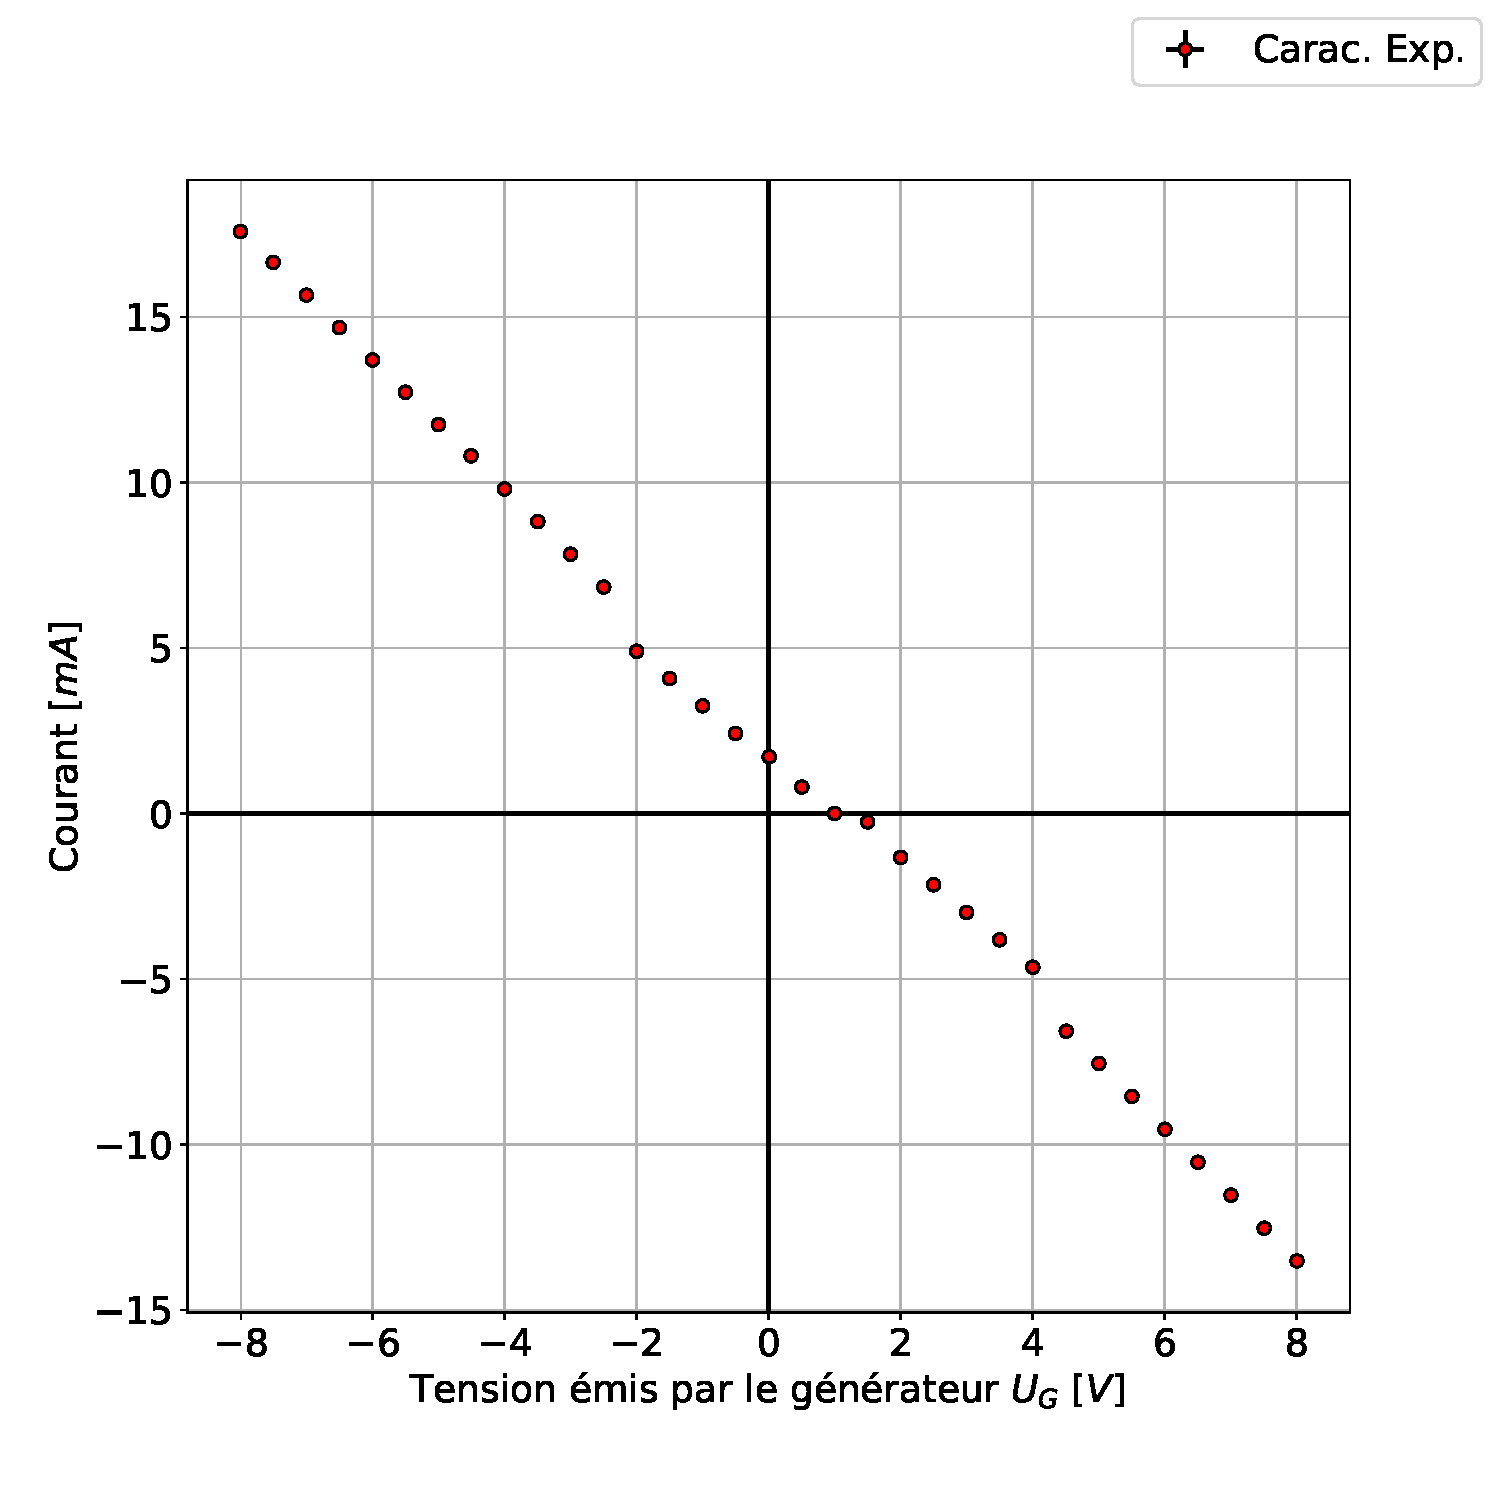
\includegraphics[width=\textwidth]{figures/Graph01a}
\end{minipage}\begin{minipage}{0.48\textwidth}
\captionof{figure}{Caractéristique expérimentale de la pile Daniell à \SI{24.9}{\celsius}.}
\end{minipage}
\end{center}
\end{solution}
\end{mybox}


\begin{mybox}
\question[2] Reproduire la fig. \ref{fig:06} et orienter les tensions électriques. Exprimer $U_G$ la tension aux bornes de la pile en fonction de la force électromotrice $U_G (I=0 ~ \si{\ampere})$, de la résistance $R$ et du courant $I$. En vous appuyant sur une des tensions mesurées précédemment, déterminer la résistance interne de la pile.
\begin{solution}[12cm]

Le modèle de Thévenin nous permet d'écrire la caractéristique de la pile comme : 
\begin{align*}
U_G (I) &= U_G(I=0) + U \\
&= U_G(I=0) - R \cdot I
\end{align*}

Dans notre expérience, on a estimé le terme résistif. Ce terme est associé à $U$ d'équation : 
\begin{align*}
U &= \Phi_{ECS_\oplus} - \Phi_{ECS_\ominus} \\ 
&= - R \cdot I
\end{align*}

On peut donc tracer la caractéristique associée à la résistance interne et la modélisée à l'aide d'une équation linéaire :
\begin{center}
\begin{minipage}{0.48\textwidth}
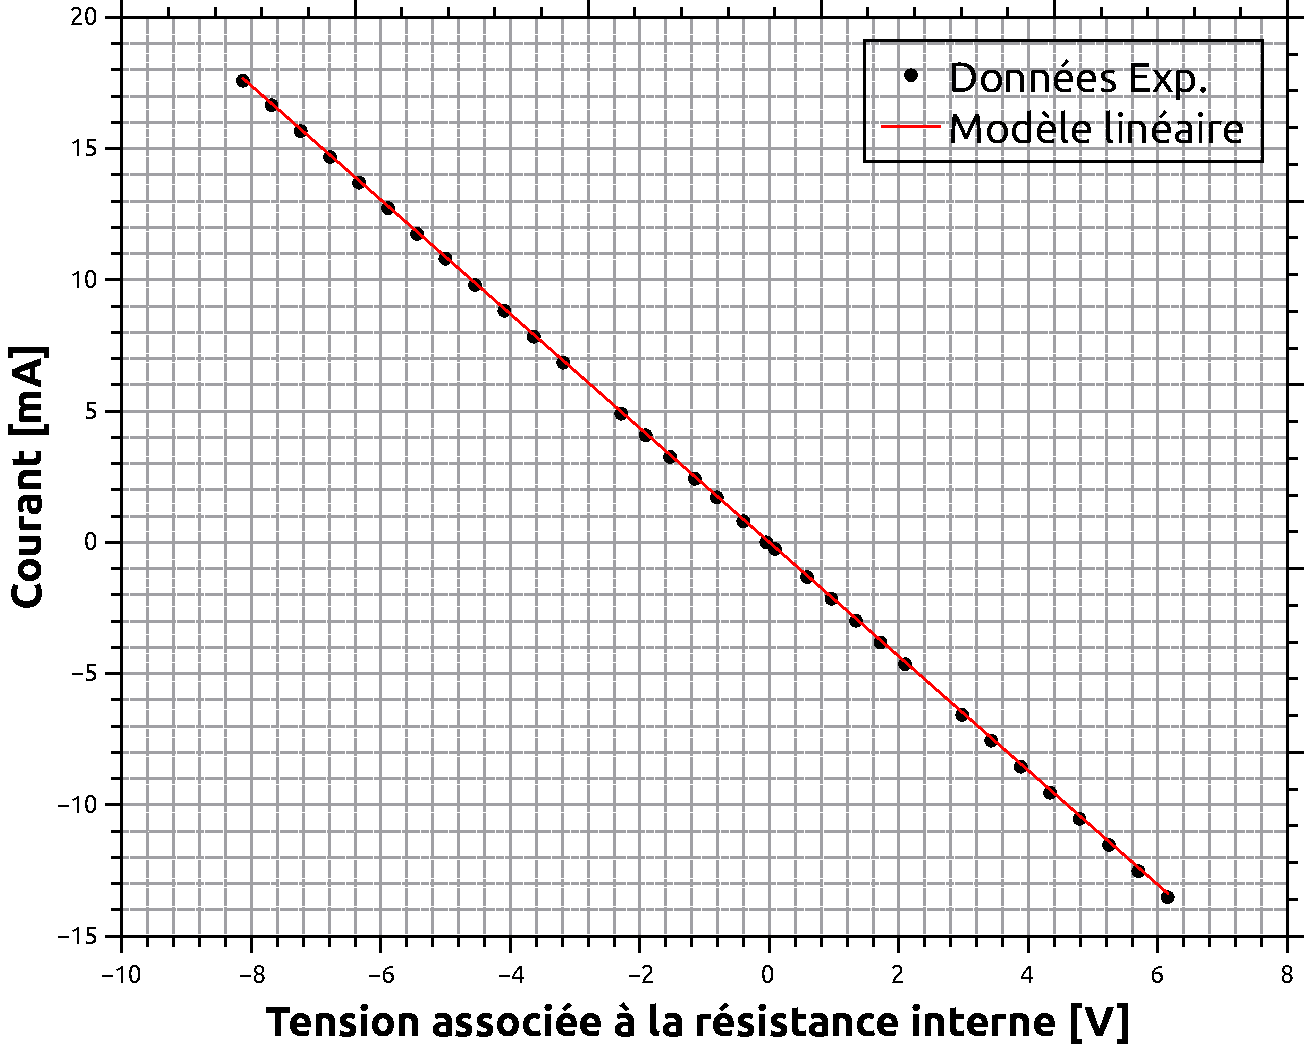
\includegraphics[width=\textwidth]{figures/Graph04}
\end{minipage}\hspace{0.2cm}\begin{minipage}{0.48\textwidth}
\captionof{figure}{Caractéristiques de la résistance interne associée à la pile Daniell maintenue à \SI{24.9}{\celsius}. Un modèle linéaire passant par (0,0) a été utilisé pour trouver la conductance.}
[Matériel : Acquisition avec un multimètre Meteix MX 554, deux électrodes de référence ECS dans les conditions de l'énoncé, analyse : Qtiplot]
\end{minipage}
\end{center}

Le modèle linéaire est partiellement validé : points alignés, $R^2 = 0.999049021\ldots$. Cependant, on remarque qu'il y a un léger biais dans la mesure du potentiel.

\begin{align*}
I [\si{\milli\ampere}] = (-2.17 \cdot 0.02) U [\si{\volt}]
\end{align*}

On trouve alors que la résistance vaut : 
\begin{align*}
R = (461 \pm 5) ~ \si{\ohm}
\end{align*}

\textbf{Nota Bene :} Les étudiants ne penseront pas à prendre en compte le biais statistique largement observé qui est dû à deux choses : 
\begin{enumerate}
\item une petite tension (biais de tension, noté $U_{biais}$) existant entre les deux ECS, laquelle a été évaluée autour de $25.4 ~ \si{\milli\volt}$ dans cette expérience ;
\item l'existence d'un potentiel de jonction $E_j$ à courant nul.
\end{enumerate}
Une modélisation de la forme : 
\begin{align*}
U - U_{biais} = E_j - R \cdot I
\end{align*}
Vous pouvez potentiellement discuter de ces paramètres avec les étudiants qui n'ont pas de difficultés. Cependant, ça ne doit pas être le c{\oe}ur de la discussion et ça ne doit pas leur faire perdre du temps.
\end{solution}
\end{mybox}

\begin{mybox}
\question[1] Superposer la caractéristique expérimentale à celle du modèle de Thévenin. En vous appuyant sur un résonnement énergétique, commenter le résultat obtenu.
\begin{solution}[8cm]
Les étudiants doivent superposer le modèle de Thévenin aux points expérimentaux :
\begin{center}
\begin{minipage}{0.48\textwidth}

\includegraphics[width=\textwidth]{figures/Graph01}
\end{minipage}\begin{minipage}{0.48\textwidth}
\captionof{figure}{Caractéristique expérimentale et d'un modèle linéaire à \SI{24.9}{\celsius}.}
\end{minipage}
\end{center}

\textbf{Interprétation du graphe :}
\begin{center}
\begin{minipage}{0.48\textwidth}
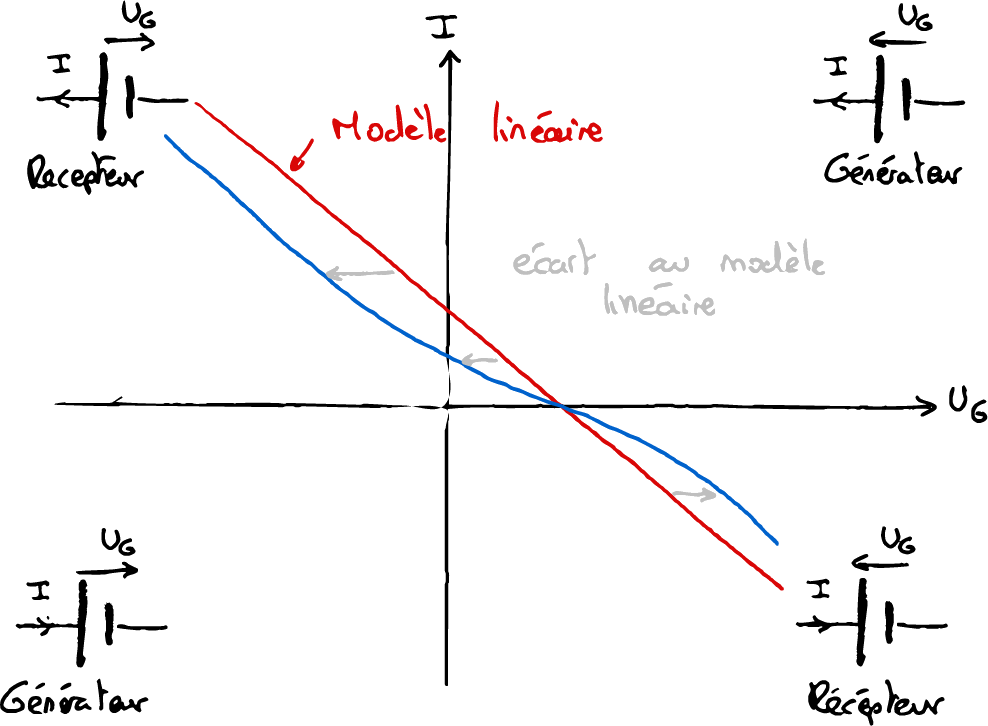
\includegraphics[width=\textwidth]{figures/Corr07}
\end{minipage}\begin{minipage}{0.48\textwidth}
\captionof{figure}{Interprétation de l'écart à linéarité.}
\end{minipage}
\end{center}


Plusieurs conclusions doivent être tirées : 
\begin{enumerate}
\item la caractéristique n'est pas du tout linéaire ;
\item la caractéristique se comporte comme suit : 
Lorsque la pile se comporte comme un générateur, à un courant donné, la tension du générateur est plus petite que la tension du modèle linéaire. Une partie de l'énergie du générateur est perdue. Lorsque la pile se comporte comme un récepteur, à un courant donné, la tension aux bornes du générateur est plus grande que la tension du modèle linéaire. Cela signifie qu'il faut fournir à la pile plus d'énergie que prédit.
\end{enumerate}
\textbf{Nota Bene :} Ne pas hésiter à aider les étudiants à bien comprendre le sens de chaque quadrant de la caractéristique. Il auront des difficultés à donner un sens "énergétique" aux tensions.
\end{solution}
\end{mybox}
\setcounter{foo}{\value{question}}
\end{questions}

Par la suite, on va chercher à comprendre l'origine chimique du terme non linéaire en représentant l'évolution des potentiels redox du cuivre et du zinc avec le courant.

\newpage

\subsubsection{\'{E}cart à la linéarité : courbe courant-potentiel}

Afin de prendre en compte l'écart à la linéarité, on va définir une nouvelle grandeur appelée surtension, qui prend en compte la différence entre le potentiel interfacial de l'électrode à courant non nul par rapport au courant nul : 
\begin{align*}
\forall I > 0, ~ E_a (I) &= E_{eq} + \eta_a (I) \quad \text{avec }\eta_a (I) > 0 \\
\forall I < 0, ~ E_c (I) &= E_{eq} + \eta_c (I) \quad \text{avec }\eta_c (I) < 0
\end{align*}
où l'indice $eq$ indique le potentiel d'équilibre, assimilable au potentiel de Nernst du couple mis en jeux dans la demi-pile et $a,c$ indique si la demi-pile est anodique ou cathodique.

Appuyez-vous sur l'annexe \ref{sec:I-E} pour répondre aux questions suivantes.

\begin{questions}
\setcounter{question}{\thefoo}
\begin{mybox}
\question[1] Représenter la courbe courant-potentiel attendu pour le cuivre et le zinc si le potentiel à chaque électrode était assimilé au potentiel thermodynamique. Vous utiliserez les conventions suivantes : 
\begin{align*}
I > 0 \implies \text{oxydation} ;\\
I < 0 \implies \text{réduction}.
\end{align*}
et vous prendre un potentiel redox exprimé en $\si{\volt\per{ECS}}$.



\begin{solution}[12cm]
Dans l'hypothèse thermodynamique, $\forall I, \quad \eta_a (I) = \eta_c (I) = 0$
\begin{align*}
E_\oplus (I) &=  E_{\oplus, eq} = E^\circ (\ce{Cu^{2+} (aq) / Cu(s)}) + \frac{\alpha}{2} \log \frac{[\ce{Cu^{2+}}]}{c^\circ} - E_{ECS} \\
E_\ominus (I) &=  E_{\ominus, eq} = E^\circ (\ce{Zn^{2+} (aq) / Zn(s)}) + \frac{\alpha}{2} \log \frac{[\ce{Zn^{2+}}]}{c^\circ} - E_{ECS}
\end{align*}
\textbf{Application Numérique :}
\begin{align*}
E_\oplus (I) &= 0.06 ~ \si{\volt\per{ECS}} \\
E_\ominus (I) &= -1.04 ~ \si{\volt\per{ECS}}
\end{align*}

On peut donc représenter la courbe courant-potentiel suivante dans un modèle \SI{100}{\percent} thermodynamique : 

\begin{center}
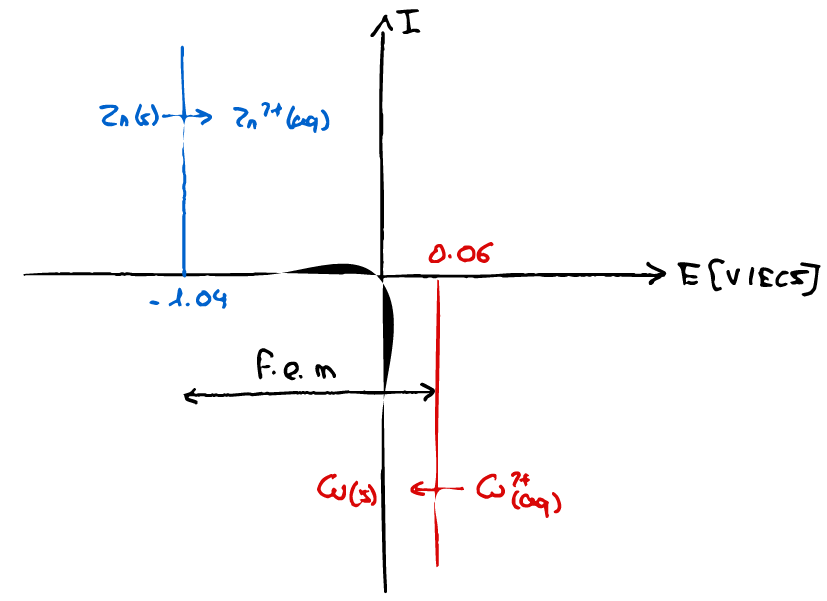
\includegraphics[width=0.48\textwidth]{figures/Corr08}
\end{center}

\end{solution}
\end{mybox}

\begin{mybox}
\question[1] Au modèle thermodynamique, vous superposerez le potentiel de chaque électrode en veillant à toujours respecter la convention suivante : 
\begin{align*}
I > 0 \implies \text{oxydation} ;\\
I < 0 \implies \text{réduction}.
\end{align*}
Représenter schématiquement les surtensions anodique $\eta_a$ et cathodique $\eta_c$ lorsque la pile fonctionne comme générateur. Quel peut-être l'origine chimique de ces surtensions ?

\begin{solution}[12cm]

Les étudiants doivent veiller à orienter leurs tensions correctement. Avec le setting expérimental utilisé, on trouve bien : 
\begin{align*}
U_G (I) &= E_{\oplus, eq} - E_{\ominus, eq} + \eta_c - \eta_a  - R \cdot I\\
&=  U_{G, Thevenin}  + \underbrace{\eta_c (I)}_{<0} - \underbrace{\eta_a (I)}_{>0} 
\end{align*}
avec $\eta_c$ (resp. $\eta_a$) la surtension cathodique (resp. anodique) du cuivre (resp. du zinc).

\begin{center}
\begin{minipage}{0.48\textwidth}
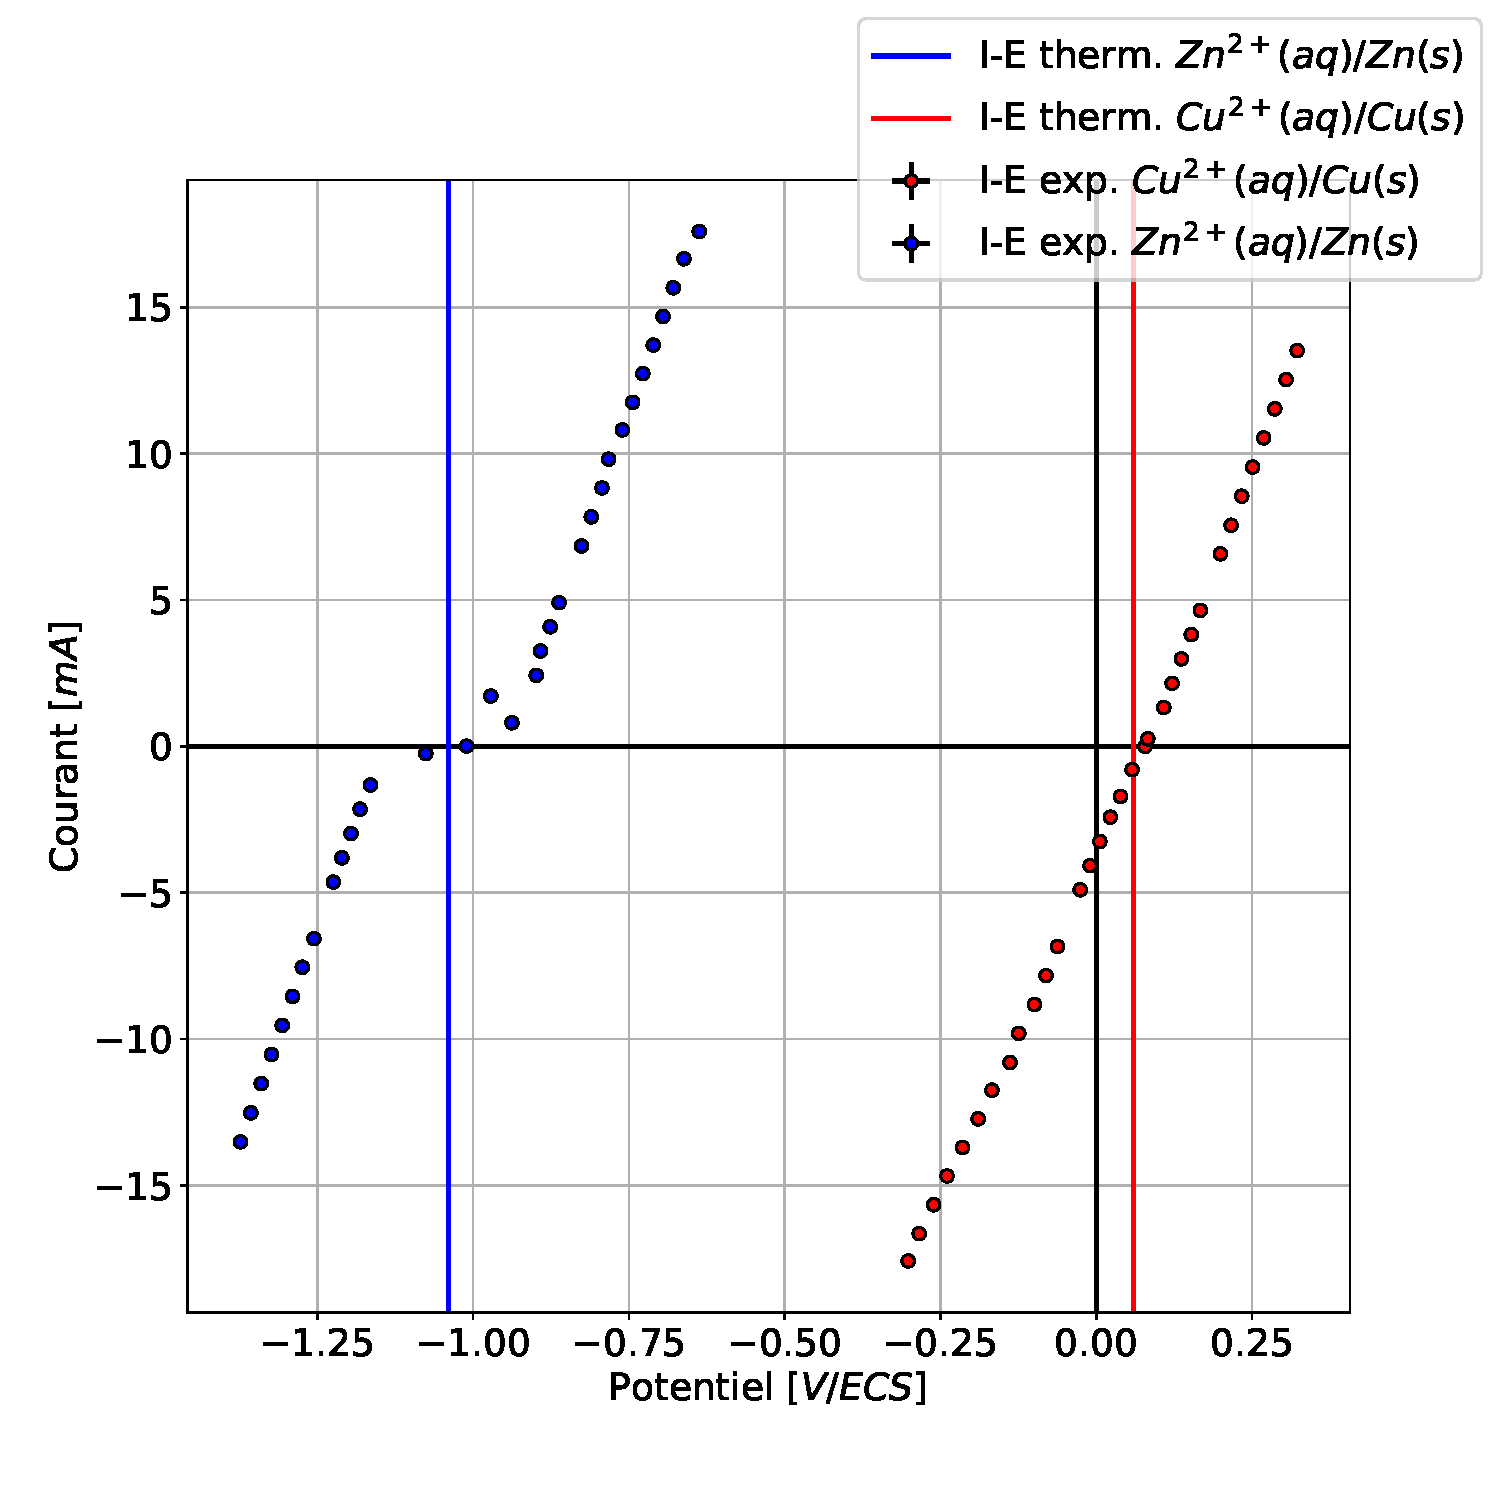
\includegraphics[width=\textwidth]{figures/Graph02}
\end{minipage}\begin{minipage}{0.48\textwidth}
\captionof{figure}{Courbe courant-potentiel à une électrode de cuivre et un électrode de zinc. Les points $\bullet$ représentent les données expérimentales, tandis que les lignes verticales représentent ce qui est prédit par la thermodynamique}
\end{minipage}
\end{center}
En ajoutant les surtensions au modèle de Thévenin, on a finalement pris en compte l'écart entre le potentiel thermodynamique et le potentiel oxydo-réduction : 
\begin{center}
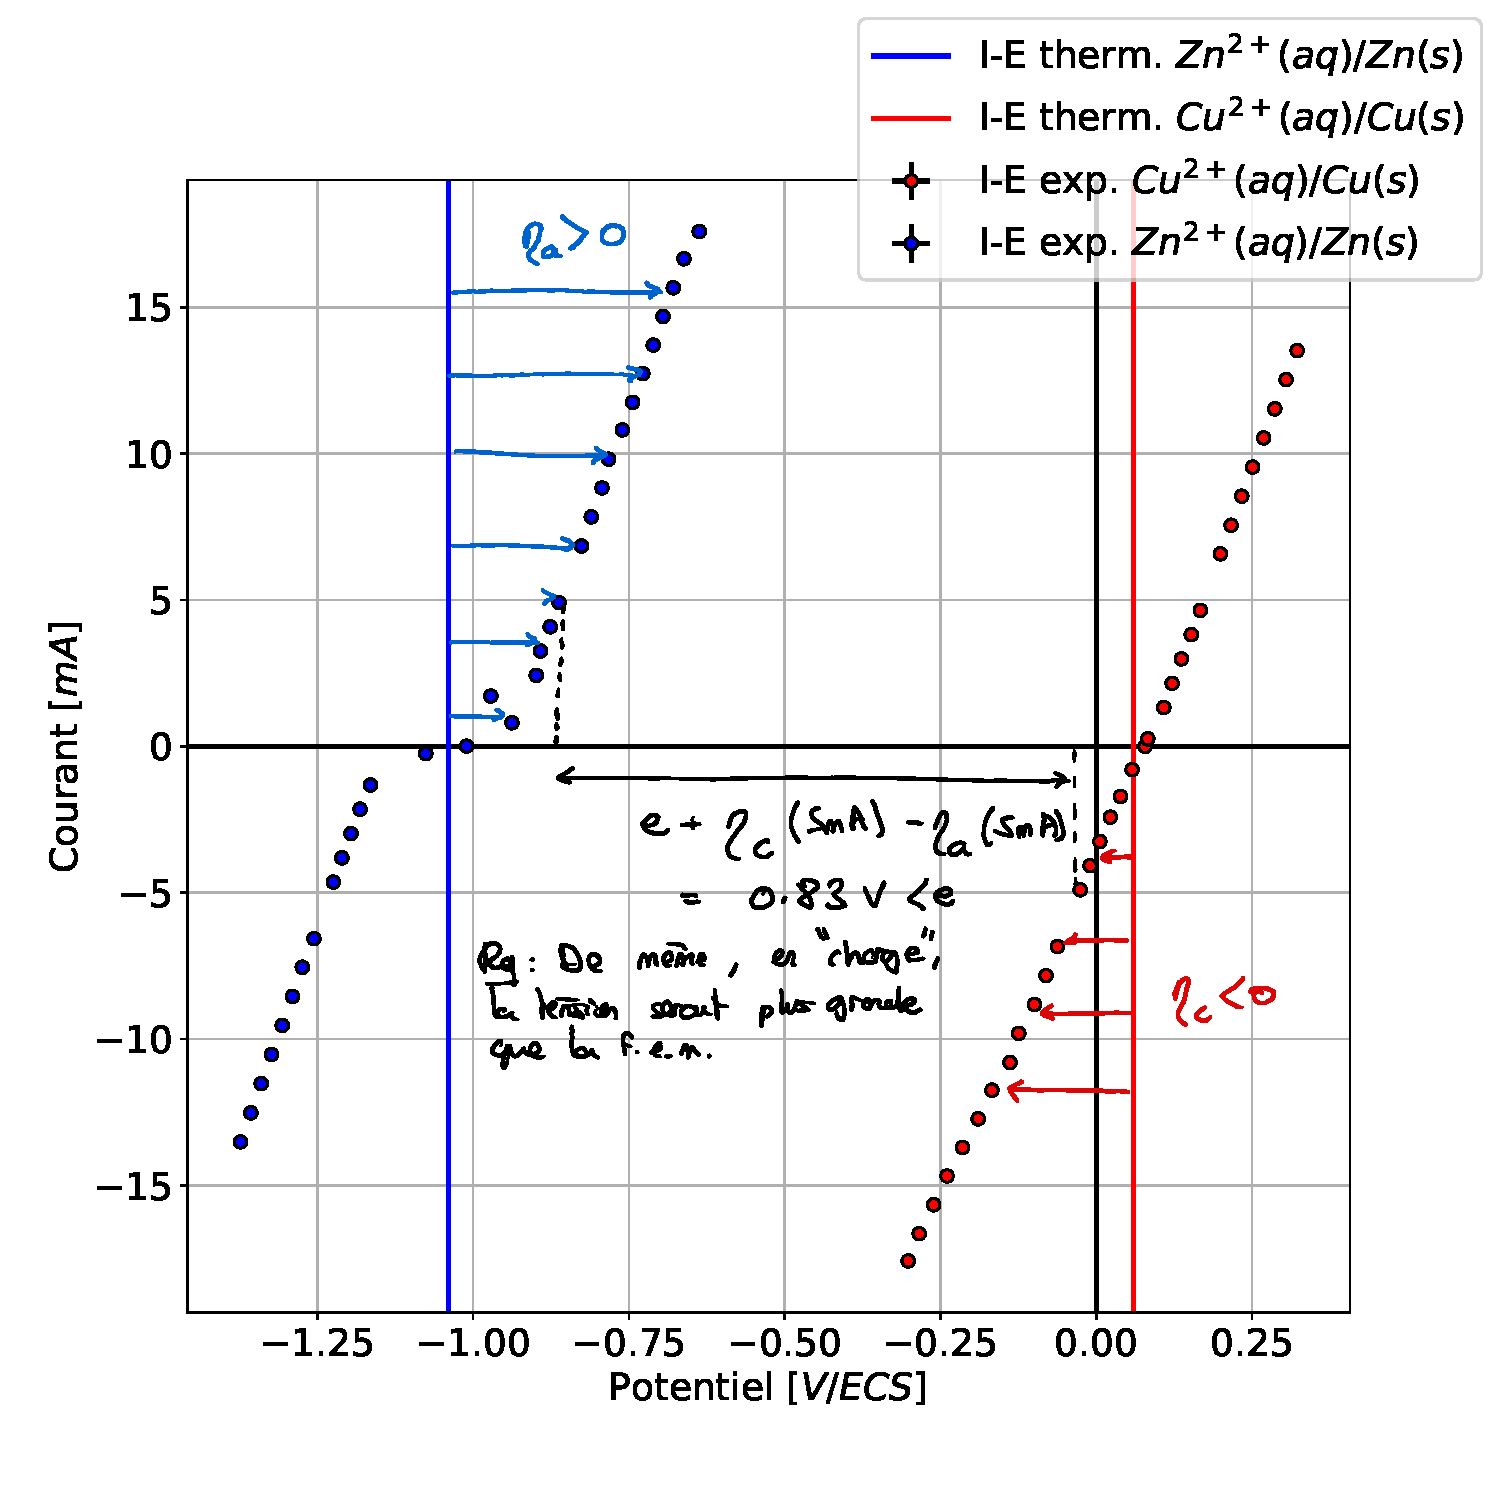
\includegraphics[width=0.48\textwidth]{figures/Graph02-bis}
\end{center}

Dans le cas du fonctionnement de la pile comme générateur, par exemple à I = \SI{5}{\milli\ampere}, la différence de potentiel entre les deux électrodes est plus faible que prédit et vaut \SI{0.83}{\volt}. Cela traduit le fait qu'une partie de l'énergie chimique libérée sert à franchir la barrière d'activation associée à l'oxydation (resp. la réduction) à la surface du zinc (resp. l'oxydation). On retrouve bien :
\begin{align*}
\forall I, U_G (I) < U_{G, Thevenin} (I)
\end{align*}

L'écart à la linéarité est d'origine \textbf{cinétique} (= phénomène d'hystérèse).
\end{solution}
\end{mybox}
\setcounter{foo}{\value{question}}
\end{questions}

\begin{comment}
Les étudiants doivent proposer un modèle type Thevenin composé d'un générateur de tension parfait et d'une résistance interne.

De ce modèle, les étudiants propose l'équation modèle suivante : 

\begin{equation*}
U_G (I)= e - R_i I \implies I (U_G) = \frac{e}{R_i} - \frac{1}{R_i} U_G
\end{equation*}
avec $e$ la tension à courant nul et $R_i$ la résistance interne.

Les étudiants pratiquent une régression linéaire et montrent que : 
\begin{itemize}
\item les points sont bien alignés ;
\item les points sont bien distribués autour de la droite ; 
\item le c{\oe}fficient de corrélation linéaire est proche de 1.
\end{itemize}
Ils concluent et valide leur modèle.

Un bonus pourra être donné à l'étudiant qui comparera la f.e.m. obtenue par le modèle à celle obtenue par une mesure directe.
\end{comment}
\newpage

\subsection{Détermination des grandeurs thermodynamiques associées à la réaction de la pile  - \faClockO ~ BONUS \si{\hour}}

On cherche à déterminer les grandeurs thermodynamiques de réaction dans la pile Zn|Cu. Pour cela, on rappelle que le comportement en température de la force électromotrice de la réaction est donnée par :

\begin{equation}
e (T) = \frac{\Delta_r S}{nF} T - \frac{\Delta_r H}{nF} 
\label{eq:e_T}
\end{equation}
avec $n$ le nombre d'électron échangé et $F$ la constante de Faraday.

Débrancher le dispositif électrique précédent et rebrancher le voltmètre, correctement orienté, aux bornes de la pile. Faites varier la température du bain de 20 à \SI{60}{\celsius}, par pas de \SI{5}{\celsius} et mesurer la tension à courant nul à chaque pas de température.

\faWarning ~ Il est inutile de perdre du temps à atteindre une équilibration à la température cible du bain. Vous pouvez annoter la température et la f.e.m. à l'aide d'un thermomètre plongé dans un compartiment de la pile.



\begin{questions}
\setcounter{question}{\thefoo}

\question[\half] Appeler l'enseignement pour qu'il vérifie le montage électrique et chimique.

\begin{mybox}
\bonusquestion[\half] \`{A} quelle condition, l'Eq. \ref{eq:e_T} donne-t-elle une droite ? 


\begin{solution}[2cm]
Si on étudie la variation de la f.e.m. sur une plage étroite de température, il se peut que le couple $(\Delta_r H, \Delta_r S)$ varie peu. Dans ce cas, on peut appliquer l'approximation d'Ellingham et considérer ces deux paramètres comme constants.
\end{solution}

\end{mybox}

\begin{mybox}
\bonusquestion[\half] En vous appuyant sur les relations démontrées à l'annexe \ref{sec:DrH&DrS}, justifier que dans la pile Daniell les grandeurs de réaction sont assimilables aux grandeurs de réaction standard : 


\begin{solution}[8cm]
Dans le cas de l'idéalité, on a $Q = \frac{[\ce{Zn^{2+}}]}{[\ce{Cu^{2+}}]}$. Puisque les deux compartiments sont théoriquement à la même concentration, et en utilisant la relation \ref{eq:DrS-DrS°}, on trouve immédiatement que :
\begin{align*}
\Delta_r S \approx \Delta_r S^\circ
\end{align*}
Avec la relation \ref{eq:DrH-DrH°}, on a aussi : 
\begin{align*}
\Delta_r H \approx \Delta_r H^\circ
\end{align*}
Par conséquent, la force électromotrice est assimilable à la force électromotrice en condition standard, et l'Eq. \ref{eq:e_T} peut se réecrire comme : 
\begin{equation}
e (T) = e^\circ (T) \approx \frac{\Delta_r S^\circ}{nF} T - \frac{\Delta_r H^\circ}{nF} 
\end{equation}

\end{solution}

\end{mybox}

\begin{mybox}
\bonusquestion[1\half] Tracer l'évolution de la f.e.m. de la pile. Appliquer cette condition et en déduire les paramètres thermodynamiques de réaction.


\begin{solution}[8cm]
La courbe obtenue est la suivante : 
\begin{center}
\begin{minipage}{0.48\textwidth}
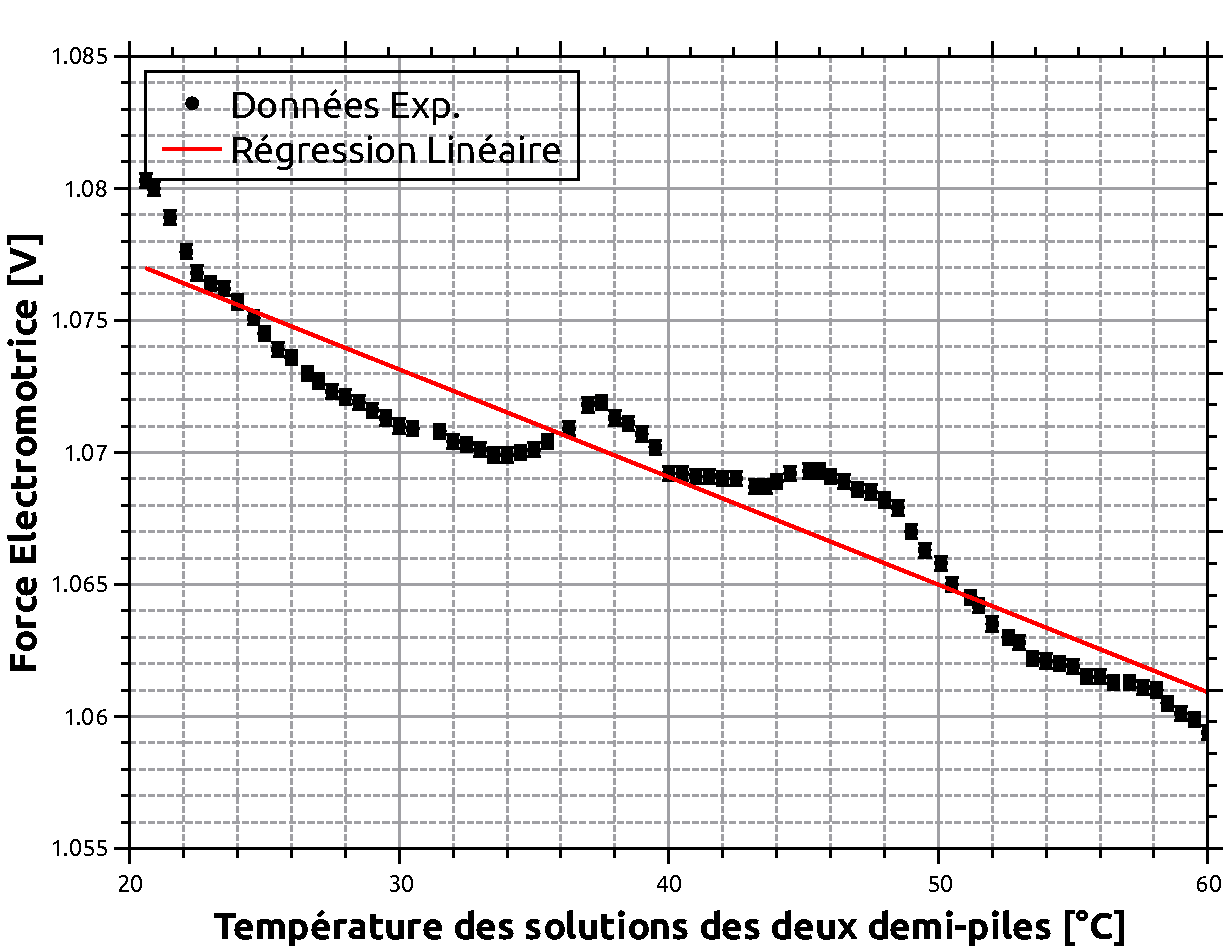
\includegraphics[width=\textwidth]{figures/Graph03}
\end{minipage}\hspace{0.2cm}\begin{minipage}{0.48\textwidth}
\captionof{figure}{\'{E}volution de la force électromotrice en fonction de la température dans un dispositif thermostaté.}
[Acquisition : multimètre Fluke 45, thermomètre Hanna HI 145 ; pile : cf. conditions opératoires, Traitement des données : Qtiplot]
\end{minipage}
\end{center}
Les étudiants tracent l'équation : 

\begin{equation*}
e^\circ (T) = \text{pente} \cdot T + \text{origine} 
\end{equation*}

avec $\text{pente} = \frac{\Delta_r S^\circ}{2F}$ et $\text{origine} = -\frac{\Delta_r H^\circ}{2F}$.

Avec les données ci-dessus, la courbe a pour équation : 
\begin{align}
e^\circ (T) (-4.1 \pm 0.2) \cdot 10^{-5} T + (1.196 \pm 0.005)
\end{align}

Encore une fois, ils valident leur modèle :
\begin{itemize}
\item en regardant la dispersion des résidus autour de la droite modèle ;
\item en regardant la distance des points à la droite modèle
\item en interprétant le $R^2$ au minimum.
\end{itemize}

Ici, on a des fluctuations surprenantes en température. Il doit y avoir un léger biais dû au contact du thermomètre avec l'électrode de zinc lors de l'acquisition. Ce biais ne devrait pas être présent avec les pièces d'acquisitions.

Cependant, le $R^2$ n'est pas trop mauvais ($\sim 0.09705$) et le $\chi^2 / dof \approx 4 \cdot 10^{-5}$ (chi2 réduit par le nombre de degré de liberté) est petit devant $1$, ce qui suggère un bon modèle de régression, mais avec des incertitudes sur-estimées. 

\begin{align*}
\Delta_r S^\circ &= (-7.9 \pm 0.4) \si{\joule\per\kelvin\per\mole} \\
\Delta_r H^\circ &= (-231 \pm 1) \si{\kilo\joule\per\mole} \\
\end{align*}
\end{solution}
\end{mybox}

\begin{mybox}
\bonusquestion[1] En vous appuyant sur les données fournies, comparer la valeur obtenue à ce que prédise les grandeurs thermodynamiques tabulées. Interpréter les éventuels écarts observés.


\begin{solution}[8cm]
Les étudiants partent de l'équation de réaction fictive : 
\begin{align*}
\ce{Zn (s) +  Cu^{2+} (aq) = Zn^{2+} (aq) + Cu (s)}
\end{align*}

et utilisent la loi de Hess : 

\begin{align*}
\Delta_r H^\circ &= \Delta_f H^\circ ( \ce{Zn^{2+} (aq)} ) - \Delta_f H^\circ ( \ce{Cu^{2+} (aq)} ) \\
\Delta_r S^\circ &= S^\circ ( \ce{Cu (s)} ) + S^\circ ( \ce{Zn^{2+} (aq)} ) - S^\circ ( \ce{Cu^{2+} (aq)} ) - S^\circ ( \ce{Zn (s)} ) 
\end{align*}

pour en déduire qu'à \SI{298}{\kelvin}, 
\begin{align*}
\Delta_r H^\circ = - 219 ~ \si{\kilo\joule\per\mole} \quad \Delta_r S^\circ = -19.9 ~ \si{\joule\per\mole\per\kelvin}
\end{align*}

On peut calculer l'écart relatif :
\begin{align}
\frac{\Delta_r H^\circ_{exp} - \Delta_r H^\circ_{theo}}{\Delta_r H^\circ_{theo}} &\approx 6 ~ \si{\percent} \\
\frac{\Delta_r S^\circ_{exp} - \Delta_r S^\circ_{theo}}{\Delta_r S^\circ_{theo}} &\approx 61 ~ \si{\percent} \\
\end{align}

On constate en somme que l'écart relatif sur l'entropie est assez grand. Ceci peut être mis en relation avec la vitesse d'acquisition de la f.e.m., laquelle n'a pas réellement été acquise en laissant le système s'équilibrer à chaque température. Avec une durée d'expérience plus longue, on pourrait potentiellement affiner la mesure.

L'écart en enthalpie est probablement dû au fait que le courant traversant la pile n'est pas tout à fait $0$, le voltmètre n'étant pas idéal. Cependant, le biais ne doit pas venir uniquement de là puisque l'on aurait sinon obtenu une f.e.m. plus petite, et donc une enthalpie plus grande que la valeur théorique. L'absence d'équilibration décrite précédemment doit aussi jouer un rôle, et compenser partiellement le biais systématique (ce qui explique la moindre erreur que l'entropie).
\end{solution}
\end{mybox}
\setcounter{foo}{\value{question}}
\end{questions}

\paragraph*{Données}
\begin{itemize}
\item constante de Faraday : $F = 96485 ~ \si{\coulomb\per\mole}$
\item valeur d'un produit de constante à \SI{298}{\kelvin} : $\alpha = RT/F \ln 10 = \SI{59}{\milli\volt}$
\item Potentiel d'une électrode au calomel saturée à \SI{298}{\kelvin} : $E_{ECS} \approx \SI{0.25}{\volt\per{ESH}}$
\item Enthalpies de formation et d'entropies molaires à \SI{298}{\kelvin} des différentes espèces impliquées dans la réaction :
\begin{center}
\begin{tabular}{cccccc}
\toprule
Espèce & & \ce{Cu(s)} & \ce{Zn(s)} & \ce{Cu^{2+} (aq)} & \ce{Zn^{2+} (aq)} \\
\midrule
$\Delta_f H^\circ$ & [\si{\kilo\joule\per\mole}] & - & - & 65 & -154 \\
$S^\circ_m$ & [\si{\joule\per\mole\per\kelvin}] & 33.5 &  41.4 & -100 & -112\\
\bottomrule
\end{tabular}
\end{center}
\item Potentiel standard en \si{\volt\per{ESH}} à \SI{298}{\kelvin} :
\begin{center}
\begin{tabular}{cccccc}
\toprule
Couple & \ce{Cu^{2+} / Cu} & \ce{Zn^{2+} / Zn} \\
\midrule
$E^\circ $ & 0.34 & -0.76 \\
\bottomrule
\end{tabular}
\end{center}
\end{itemize}

\begin{comment}
\begin{center}
\begin{tabular}{cccccc}
Espèce & & \ce{Al(s)} & \ce{Ag(s)} & \ce{Al^{3+} (aq)} & \ce{Ag^+ (aq)} \\
$\Delta_f H^\circ$ & [\si{\kilo\joule\per\mole}] & - & - & -531 & 106 \\
$S^\circ_m$ & [\si{\joule\per\mole\per\kelvin}] & 33 & 54 & -322 & 73\\
\end{tabular}
\end{center}
\end{comment}

\newpage

\appendix

\section{Produits chimiques}

\subsection{\'{E}chelle de potentiel}

\begin{center}
\begin{tabular}{|C{3cm}|C{3cm}|c|C{6cm}|}
\hline
Produit & Données & Pictogrammes & Mention de danger \\
\hline
Cuivre & - & - & -\\
\hline
Zinc & - & - & -\\
\hline
Aluminium & - & - & -\\
\hline
Argent & - & - & -\\
\hline
Fer & - & - & -\\
\hline
Solution de sulfate de cuivre & \SI{0.01}{\mole\per\liter} & 
\includegraphics[width=1cm]{pictos/exclam.pdf}
\includegraphics[width=1cm]{pictos/envi.pdf} & H319 Provoque une sévère irritation des yeux ; H411 Toxique pour les organismes aquatiques, entraîne des effets néfastes à long terme\\
\hline
Solution de sulfate de zinc & \SI{0.01}{\mole\per\liter} & 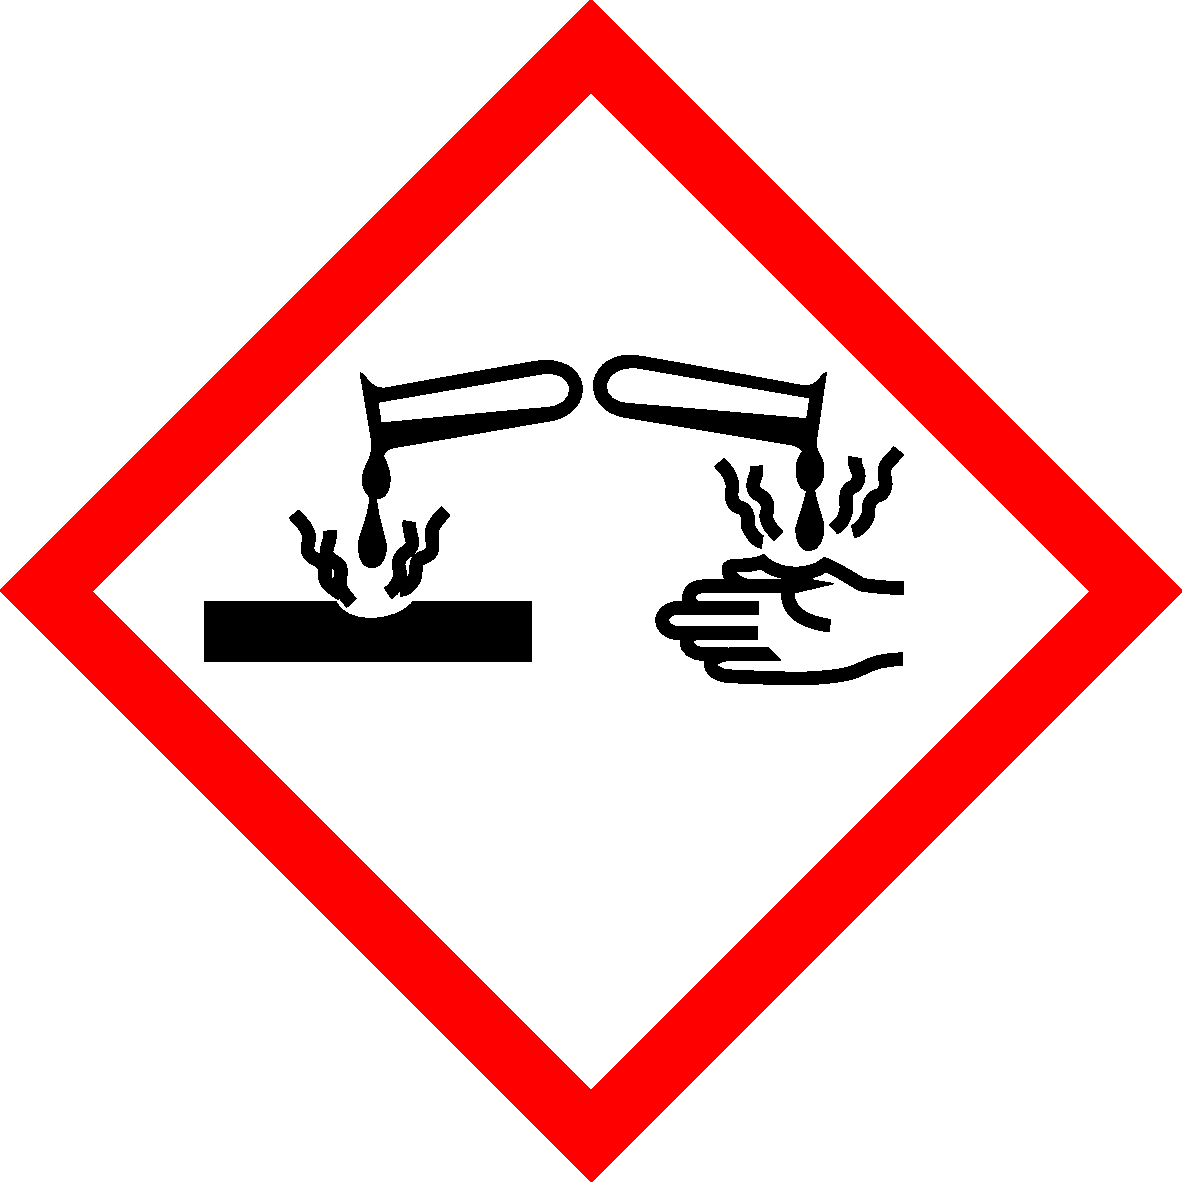
\includegraphics[width=1cm]{pictos/corro.pdf}
\includegraphics[width=1cm]{pictos/envi.pdf} & H290 Peut être corrosif pour les métaux ; H318 Provoque de graves lésions des yeux ; H411 Toxique pour les organismes aquatiques, entraîne des effets
néfastes à long terme.\\
\hline
%Sulfate d'aluminium (\SI{0.01}{\mole\per\liter}) & - & 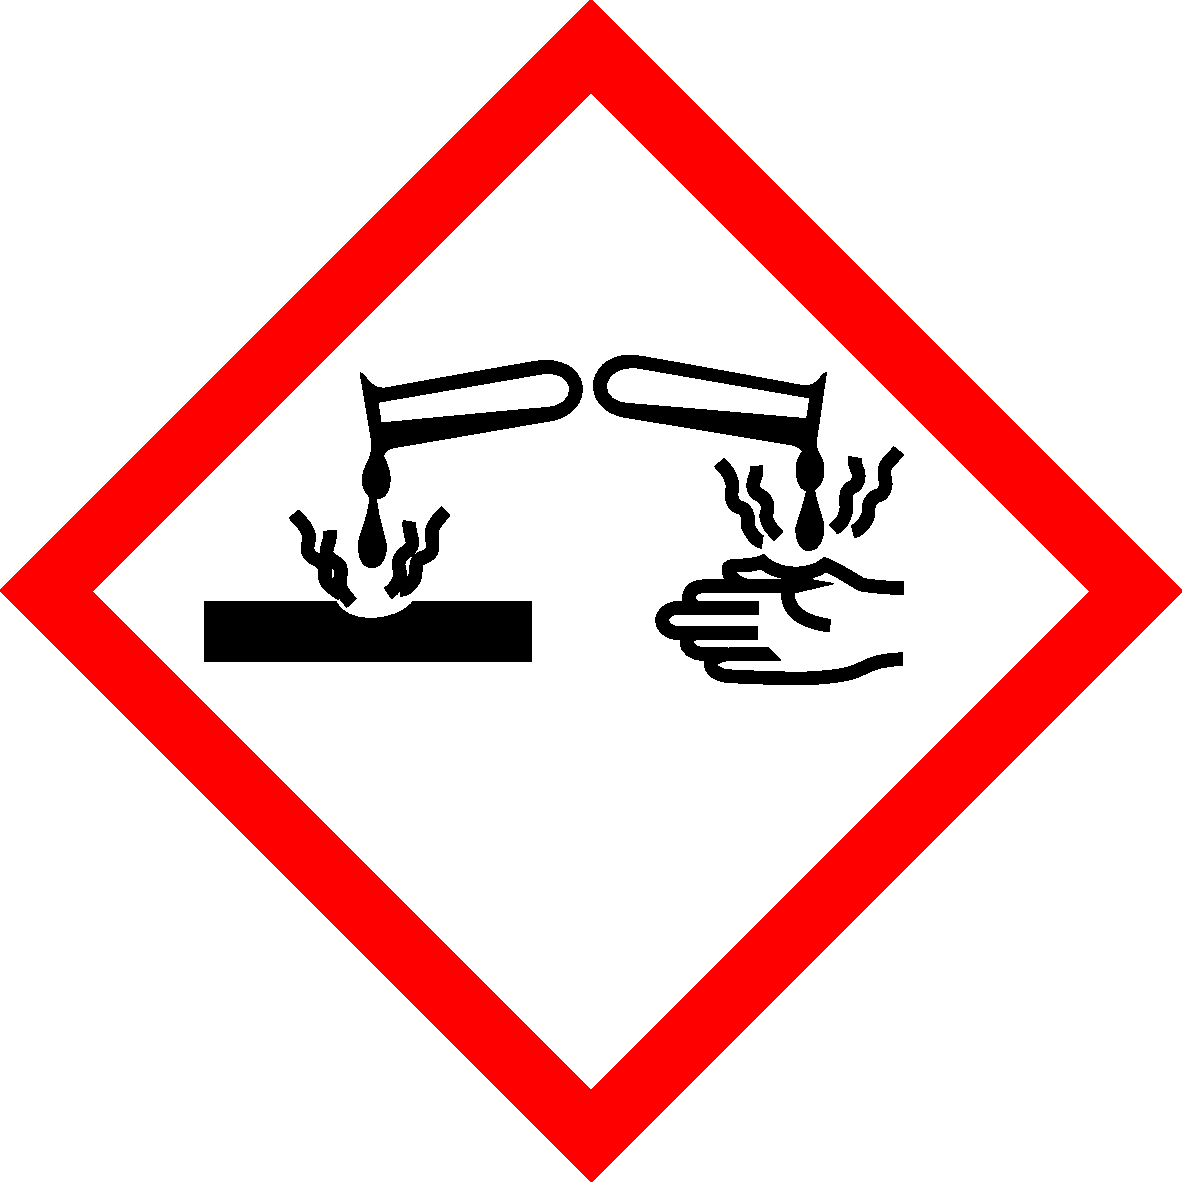
\includegraphics[width=1cm]{pictos/corro.pdf} & H314 : Provoque de graves brûlures de la peau et de graves lésions des yeux ; H290 Peut être corrosif pour les métaux.\\
Nitrate d'aluminium & \SI{0.01}{\mole\per\liter} & 
\includegraphics[width=1cm]{pictos/combu.pdf}
\includegraphics[width=1cm]{pictos/exclam.pdf} & H272 : Peut aggraver un incendie, comburant ; H315 : Provoque une irritation cutanée ; H319 : Provoque une sévère irritation des yeux\\
\hline
Nitrate d'argent & \SI{0.01}{\mole\per\liter} & 
\includegraphics[width=1cm]{pictos/combu.pdf}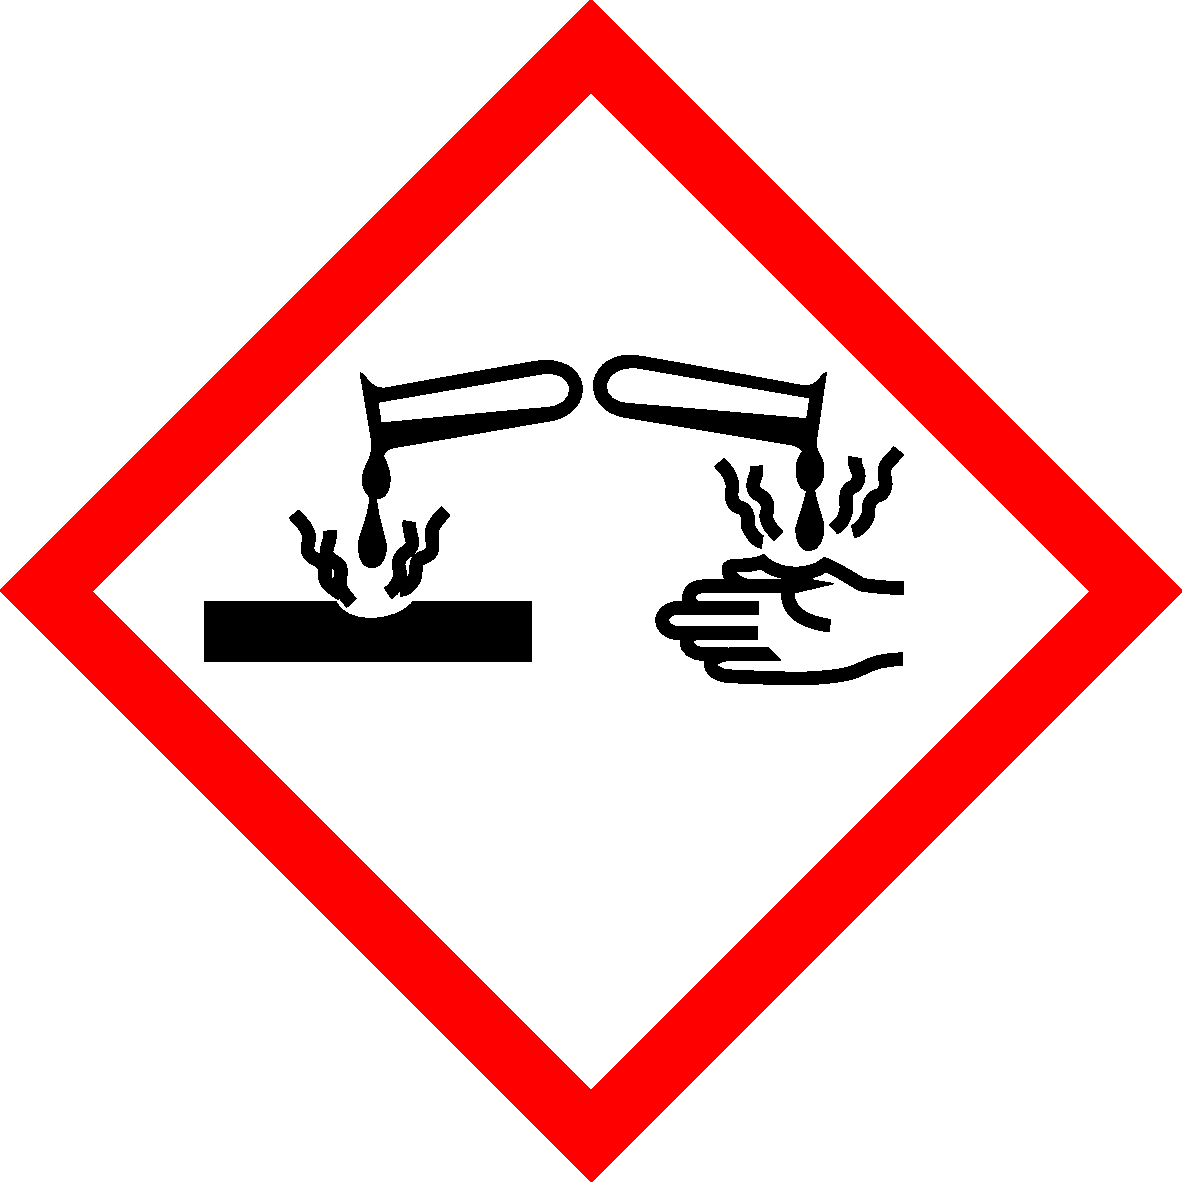
\includegraphics[width=1cm]{pictos/corro.pdf}
\includegraphics[width=1cm]{pictos/envi.pdf} & H272 Peut aggraver un incendie, comburant ; H314 : Provoque de graves brûlures de la peau et des lésions oculaires ; H290 : Peut être corrosif pour les métaux ; H400 : Très toxique pour les organismes aquatiques ; H410 : Très toxique pour les organismes aquatiques, entraîne des effets à long terme\\
\hline
Sulfate de fer (II) & \SI{0.01}{\mole\per\liter} & 
\includegraphics[width=1cm]{pictos/exclam.pdf} & H302 Nocif en cas d'ingestion ;  	H315 Provoque une irritation cutanée ; H319 Provoque une sévère irritation des yeux \\
\hline
\end{tabular}
\end{center}



\subsection{Détermination de grandeurs thermodynamique et cinétique de cellules électrochimiques}

\begin{center}
\begin{tabular}{|C{3cm}|C{3cm}|c|C{6cm}|}
\hline
Produit & Données & Pictogrammes & Mention de danger \\
\hline
Solution de sulfate de cuivre & \SI{0.1}{\mole\per\liter} & 
\includegraphics[width=1cm]{pictos/exclam.pdf}
\includegraphics[width=1cm]{pictos/envi.pdf} & H319 Provoque une sévère irritation des yeux ; H411 Toxique pour les organismes aquatiques, entraîne des effets néfastes à long terme\\
\hline
Solution de sulfate de zinc &  \SI{0.1}{\mole\per\liter} & 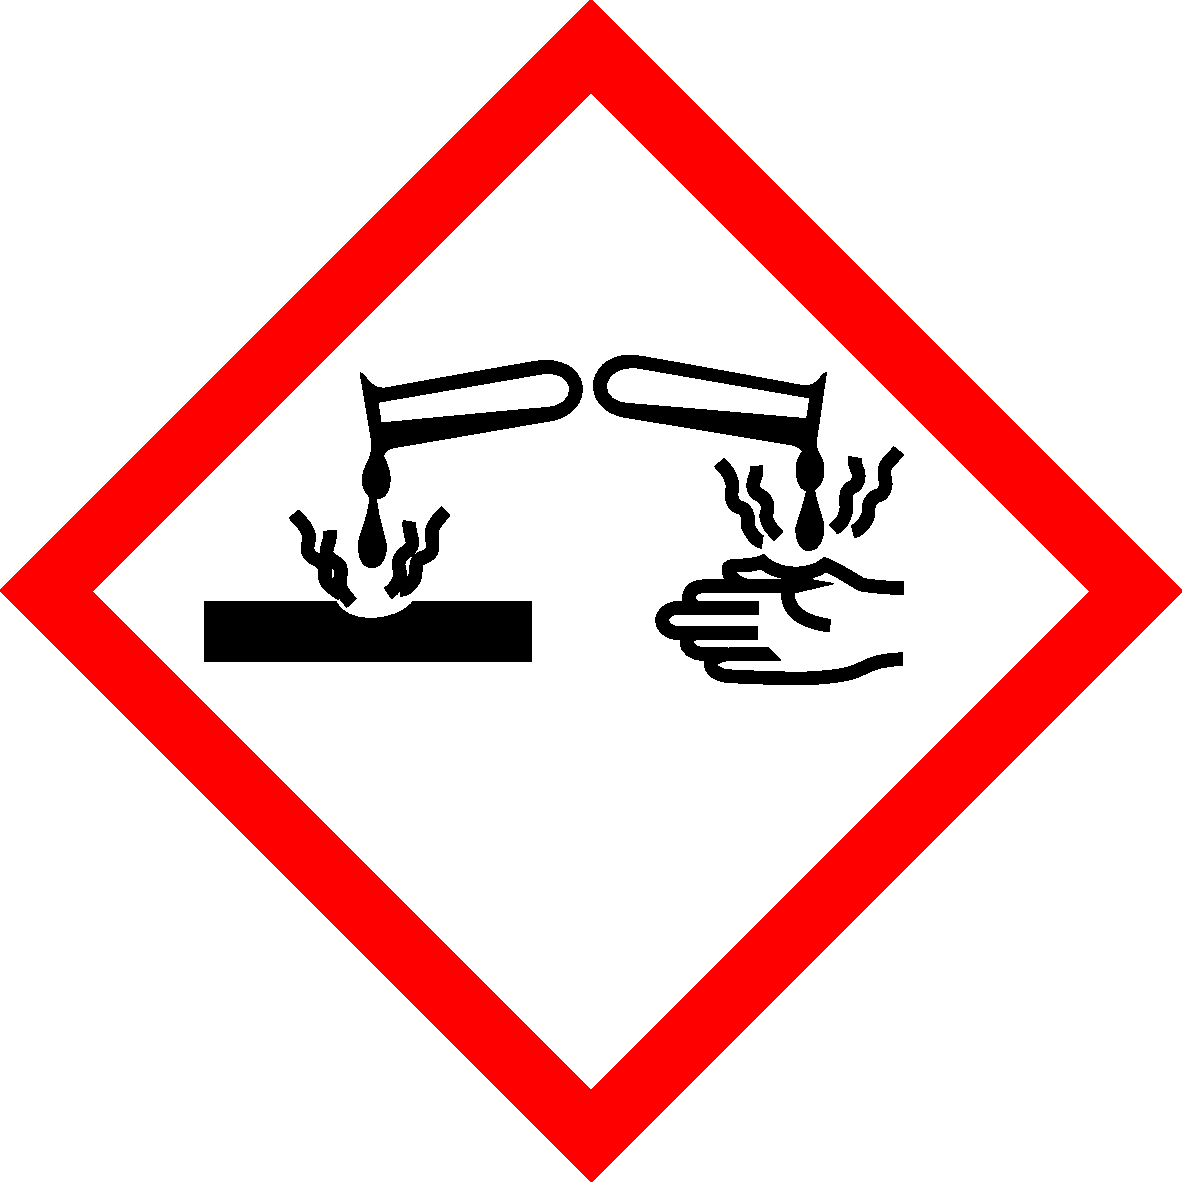
\includegraphics[width=1cm]{pictos/corro.pdf}
\includegraphics[width=1cm]{pictos/envi.pdf} & H290 Peut être corrosif pour les métaux ; H318 Provoque de graves lésions des yeux ; H411 Toxique pour les organismes aquatiques, entraîne des effets
néfastes à long terme.\\
\hline
Cuivre & - & - & -\\
\hline
Zinc & - & - & -\\
\hline
\end{tabular}
\end{center}

\section{Grandeurs de réaction dans les conditions standard}
\label{sec:DrH&DrS}

Dans cette annexe, on fournit les démonstrations thermodynamiques sur lesquelles vous pouvez vous appuyez pour assimiler les grandeurs de réaction mesurées en condition ambiante aux grandeurs en condition standard.

Dans le cas de l'entropie, on part de la définition de l'entropie à pression constante : 

\begin{align}
\left( \frac{\partial G}{\partial T} \right)_{P, \xi} = - S \label{eq:def_S}
\end{align}

En utilisant la relation de Schwartz et en dérivant partiellement selon $\xi$, on a : 
\begin{align}
\left( \frac{\partial \Delta_r G}{\partial T} \right)_{P, \xi} = - \Delta_r S
\end{align}

Or on sait exprimer l'enthalpie libre de réaction : 
\begin{align}
\Delta_r G = \Delta_r G^\circ (T) + RT \ln Q
\label{eq:DrG}
\end{align}

On peut dériver partiellement l'Eq. \ref{eq:DrG} par rapport à la température : 
\begin{align}
\left( \frac{\partial}{\partial T} (\Delta_r G^\circ (T) + RT \ln Q) \right)_{P, \xi} &= - \Delta_r S \\
\left( \frac{\partial}{\partial T} \Delta_r G^\circ (T)\right)_{P, \xi}  + R \ln Q   &= - \Delta_r S \\
-\Delta_r S^\circ  + R \ln Q  &= - \Delta_r S \\
\Delta_r S^\circ  - R \ln Q  &= \Delta_r S \label{eq:DrS-DrS°}
\end{align}
L'Eq. \ref{eq:DrS-DrS°} permet de lier l'entropie de réaction à la grandeur équivalente en condition standard

Pour ce qui est l'enthalpie, il faut utiliser une astuce en partant de la définition de G : 
\begin{align}
G &= H - T S \\
G &= H + \left( \frac{\partial G}{\partial T} \right)_{P, \xi} T \quad \text{en utilisant l'Eq.}\ref{eq:def_S} \\
\frac{G}{T^2} &= \frac{H}{T^2} + \frac{1}{T} \left( \frac{\partial G}{\partial T} \right)_{P, \xi} \\
- \frac{G}{T^2} + \frac{1}{T} \left( \frac{\partial G}{\partial T} \right)_{P, \xi} &= - \frac{H}{T^2} \label{eq:pre_GibbsHelmholtz}
\end{align}
Dans l'Eq. \ref{eq:pre_GibbsHelmholtz}, le terme à gauche est la dérivée partielle du produit G/T par rapport à la température, soit : 
\begin{align}
\left( \frac{\partial \frac{G}{T}}{\partial T} \right)_{P, \xi} = - \frac{H}{T^2}
\end{align}
En utilisant le théorème de Schwartz et en dérivant partiellement selon $\xi$, on a : 
\begin{align}
\left( \frac{\partial \frac{\Delta_r G}{T}}{\partial T} \right)_{P, \xi} = - \frac{\Delta_r H}{T^2}
\end{align}
On peut alors juste utiliser l'Eq. \ref{eq:DrG} :
\begin{align}
\left( \frac{\partial \frac{\Delta_r G^\circ}{T} + R \ln Q}{\partial T} \right)_{P, \xi} &= - \frac{\Delta_r H}{T^2} \\
\left( \frac{\partial \frac{\Delta_r G^\circ}{T}}{\partial T} \right)_{P, \xi} &\approx - \frac{\Delta_r H}{T^2} \\
- \frac{\Delta_r H^\circ}{T^2} &\approx - \frac{\Delta_r H}{T^2} \implies  \Delta_r H \approx \Delta_r H^\circ \label{eq:DrH-DrH°}
\end{align}
L'Eq. \ref{eq:DrH-DrH°} montre que l'enthalpie de réaction s'assimile assez bien à l'enthalpie standard de réaction.

\section{Courbes courant-potentiel}
\label{sec:I-E}

{\tiny La résistance interne de la cellule électrochimique sera négligée dans les explications ci-dessous pour un intérêt purement pédagogique.}% M. Olivieri se décharge de toute responsabilité sur les conséquences sur le cerveau des étudiants.}

Un des outils les plus utilisés permettant de décrire la thermodynamique et la cinétique des réactions de transfert d'électron (redox) ayant lieu à la surface des électrodes est la \textbf{courbe courant-potentiel}.

Considérons une batterie en décharge, où dans chaque compartiment, on a les réactions suivantes : 

\begin{center}
\begin{minipage}{0.5\textwidth}
\begin{align*}
\ce{Red (\ominus) &-> Ox (\ominus) + e^-} \\
\ce{Ox (\oplus) + e^- &-> Red (\oplus)} \\
\hline
\ce{Ox (\oplus) + Red (\ominus) &-> Red (\oplus) + Ox (\ominus)}
\end{align*}
\end{minipage}
\end{center}

Dans un monde idéal, le transfert d'électron serait infiniment rapide (instantanée). Dans ce cas, à tout courant et à chaque électrode, le potentiel d'électrode resterait constant et garderait la valeur prédit à l'équilibre (par la thermodynamique) :
\begin{align*}
\forall I, \quad E_i(I) = E_{i,eq}
\end{align*}
avec $i=\oplus$ ou $\ominus$ et $eq$ signifie qu'il s'agit de la valeur à l'équilibre thermodynamique (calculable via la relation de Nernst).

Dans ce cas idéal, la courbe i-E aurait l'allure suivante : 
\begin{figure}[H]
\begin{minipage}{0.58\textwidth}
\subfloat[\label{fig:Ann02a}]{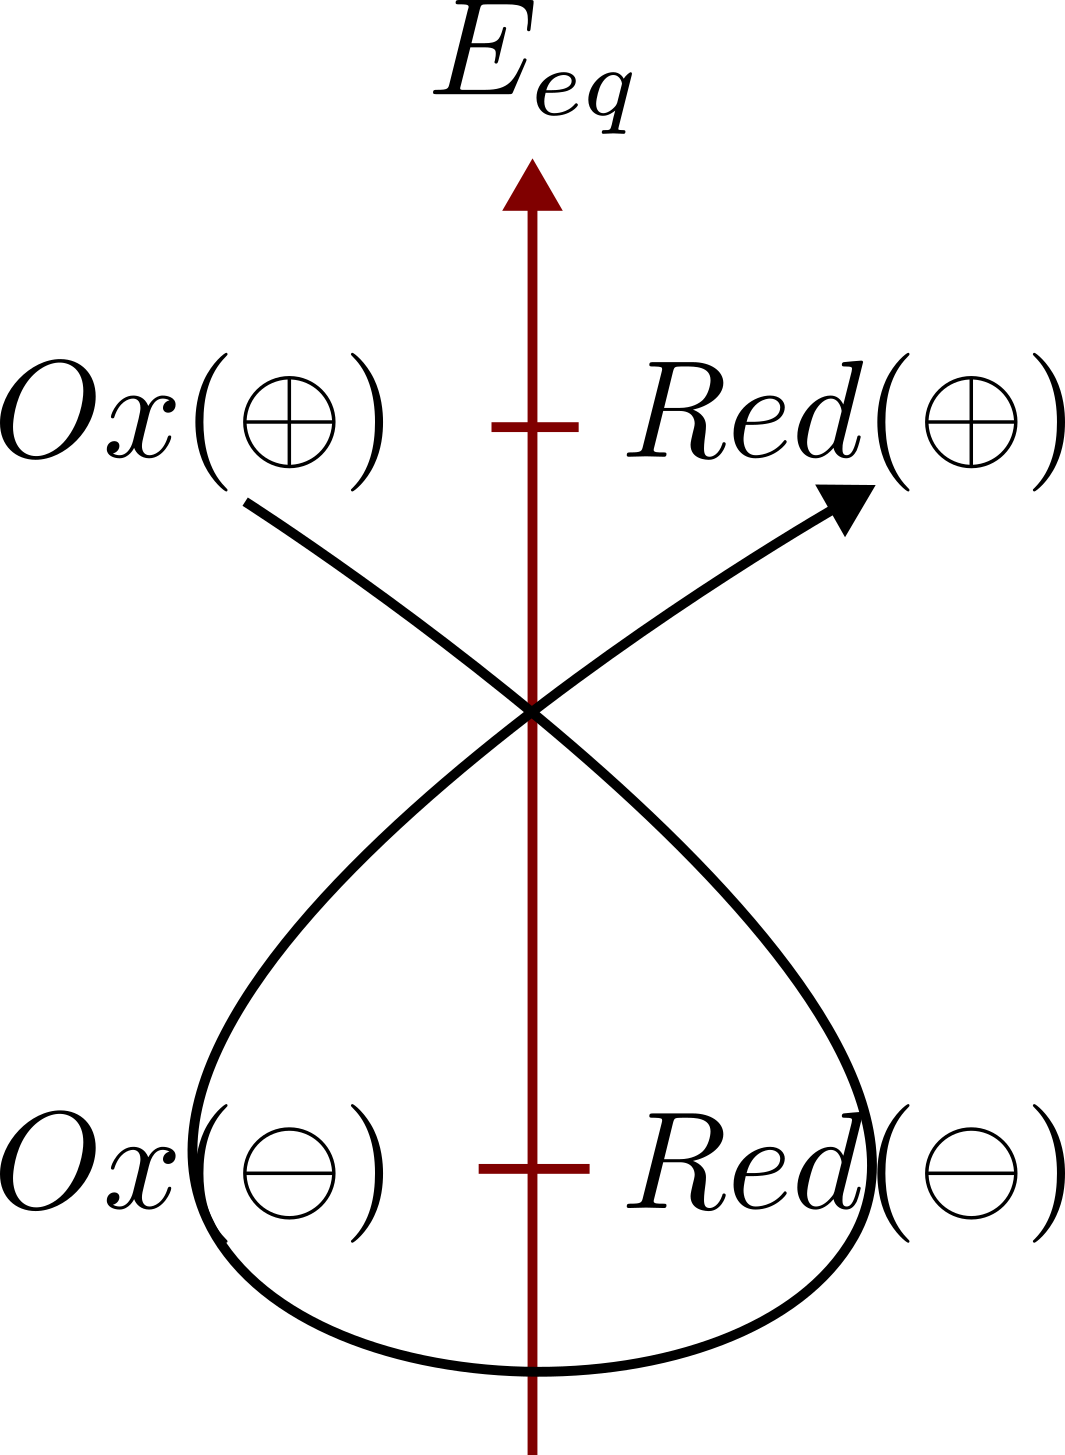
\includegraphics[height=4cm]{figures/Ann02a}}\hfill
\subfloat[\label{fig:Ann02b}]{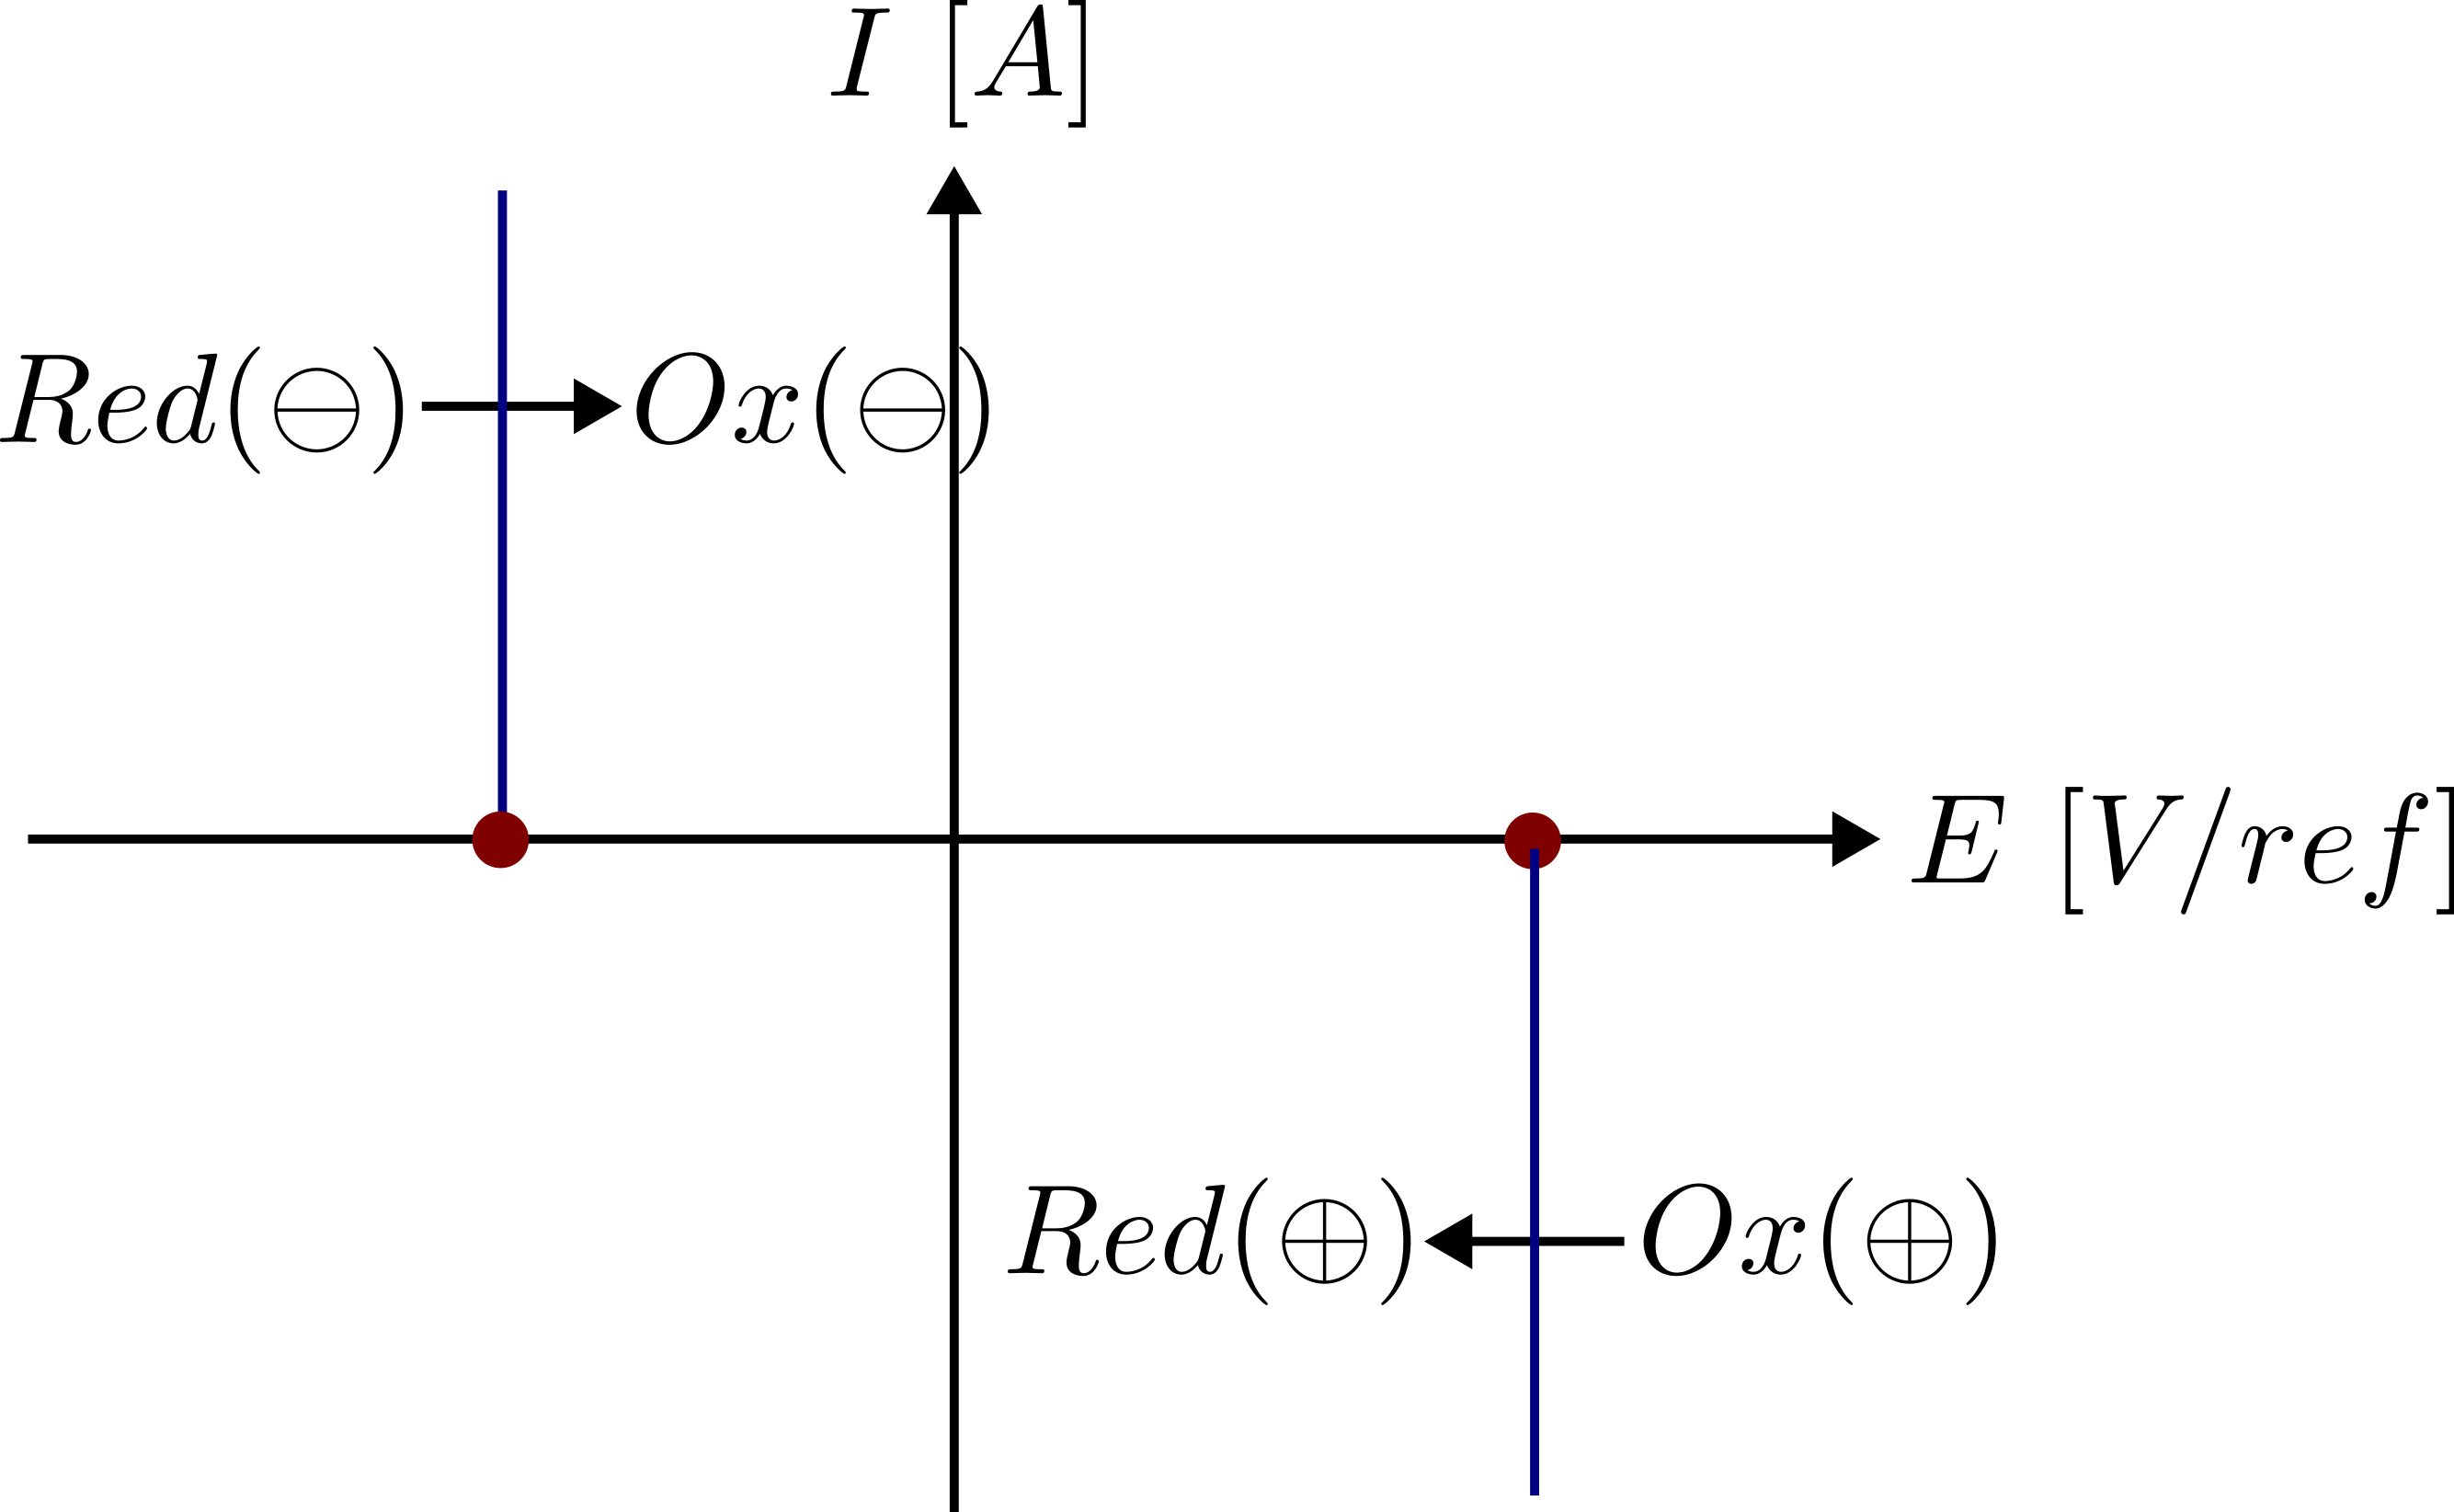
\includegraphics[height=4cm]{figures/Ann02b}}
\end{minipage}\begin{minipage}{0.38\textwidth}
\caption{\ref{fig:Ann02a} Axe de potentiel thermodynamique ; \ref{fig:Ann02b} Courbe courant-potentiel dans le cas idéal où le transfert d'électron serait infiniment rapide, construite à partir de l'axe de potentiel thermodynamique en utilisant la convention $I>0$ : oxydation, $I<0$ : réduction}
\end{minipage}
\end{figure}

Dans le monde idéal, la tension aux bornes de la pile serait constante et serait donnée par : 
\begin{align*}
U = E_{eq, \oplus} - E_{eq, \ominus}
\end{align*}



Malheureusement pour nous, les réactions chimiques ont lieu à une vitesse de réaction finie. De plus, il faut fournir une certaine énergie pour que le transfert de réaction ait lieu à une vitesse non nulle !

Les électrochimistes définissent les \textbf{surtensions}, exprimées en volt, qui sont des paramètres liés à l'énergie d'activation de chacune des réactions de transfert d'électron. Ce sont des fonctions du courant $I$ qui mesure l'écart à la thermodynamique : 
\begin{align*}
\eta_a (I)= E_a (I) - E_{a,eq} \\
\eta_c (I) = E_c (I) - E_{c,eq} \\
\end{align*}
avec $a,c$ signifiant anodique et cathodique. 

\faWarning ~ Les surtensions sont définies pour un couple donné et une électrode donné et dépendent de la nature des réactions du transfert chimique (oxydation=anode, réduction=cathode) plutôt que du pôle. A tout courant, on aura toujours $\eta_a (I) > 0$ et $\eta_c (I) < 0$.

On a alors deux cas possible qui dépendent si la cellule électrochimique est en charge ou en décharge : 

\begin{figure}[H]
\begin{minipage}{0.78\textwidth}
\subfloat[\label{fig:Ann03a}]{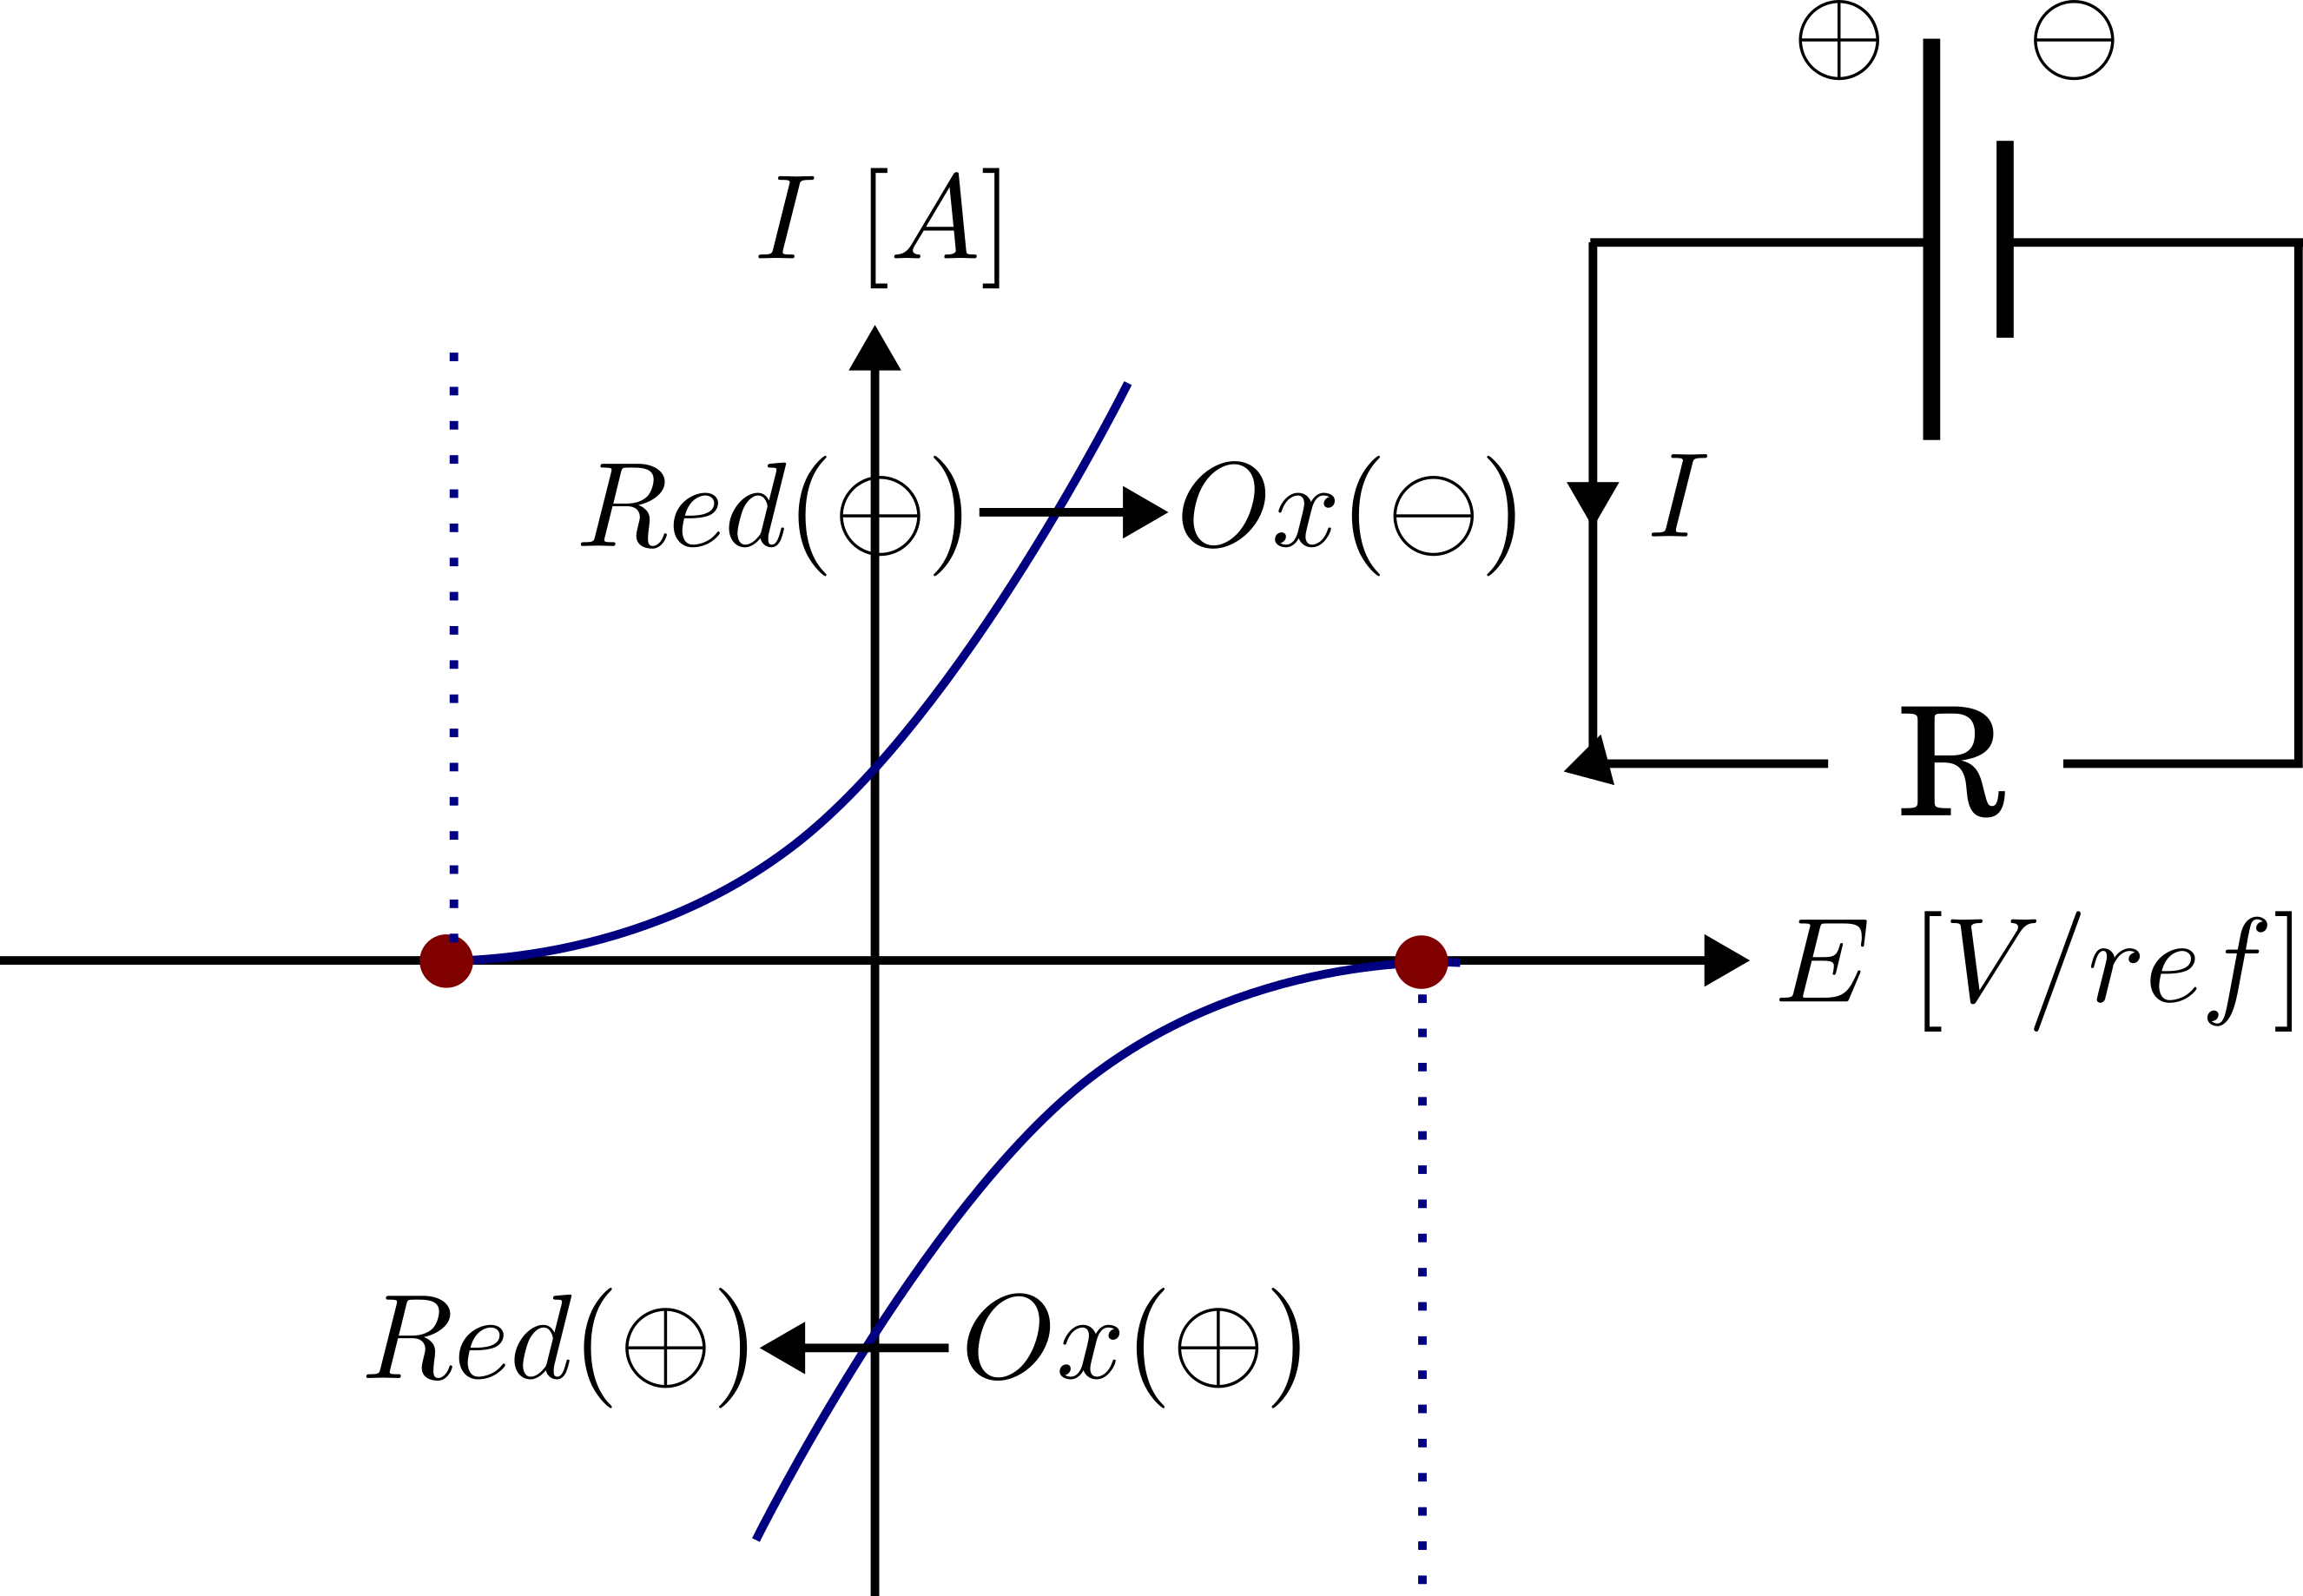
\includegraphics[height=4cm]{figures/Ann03a}}\hfill
\subfloat[\label{fig:Ann03b}]{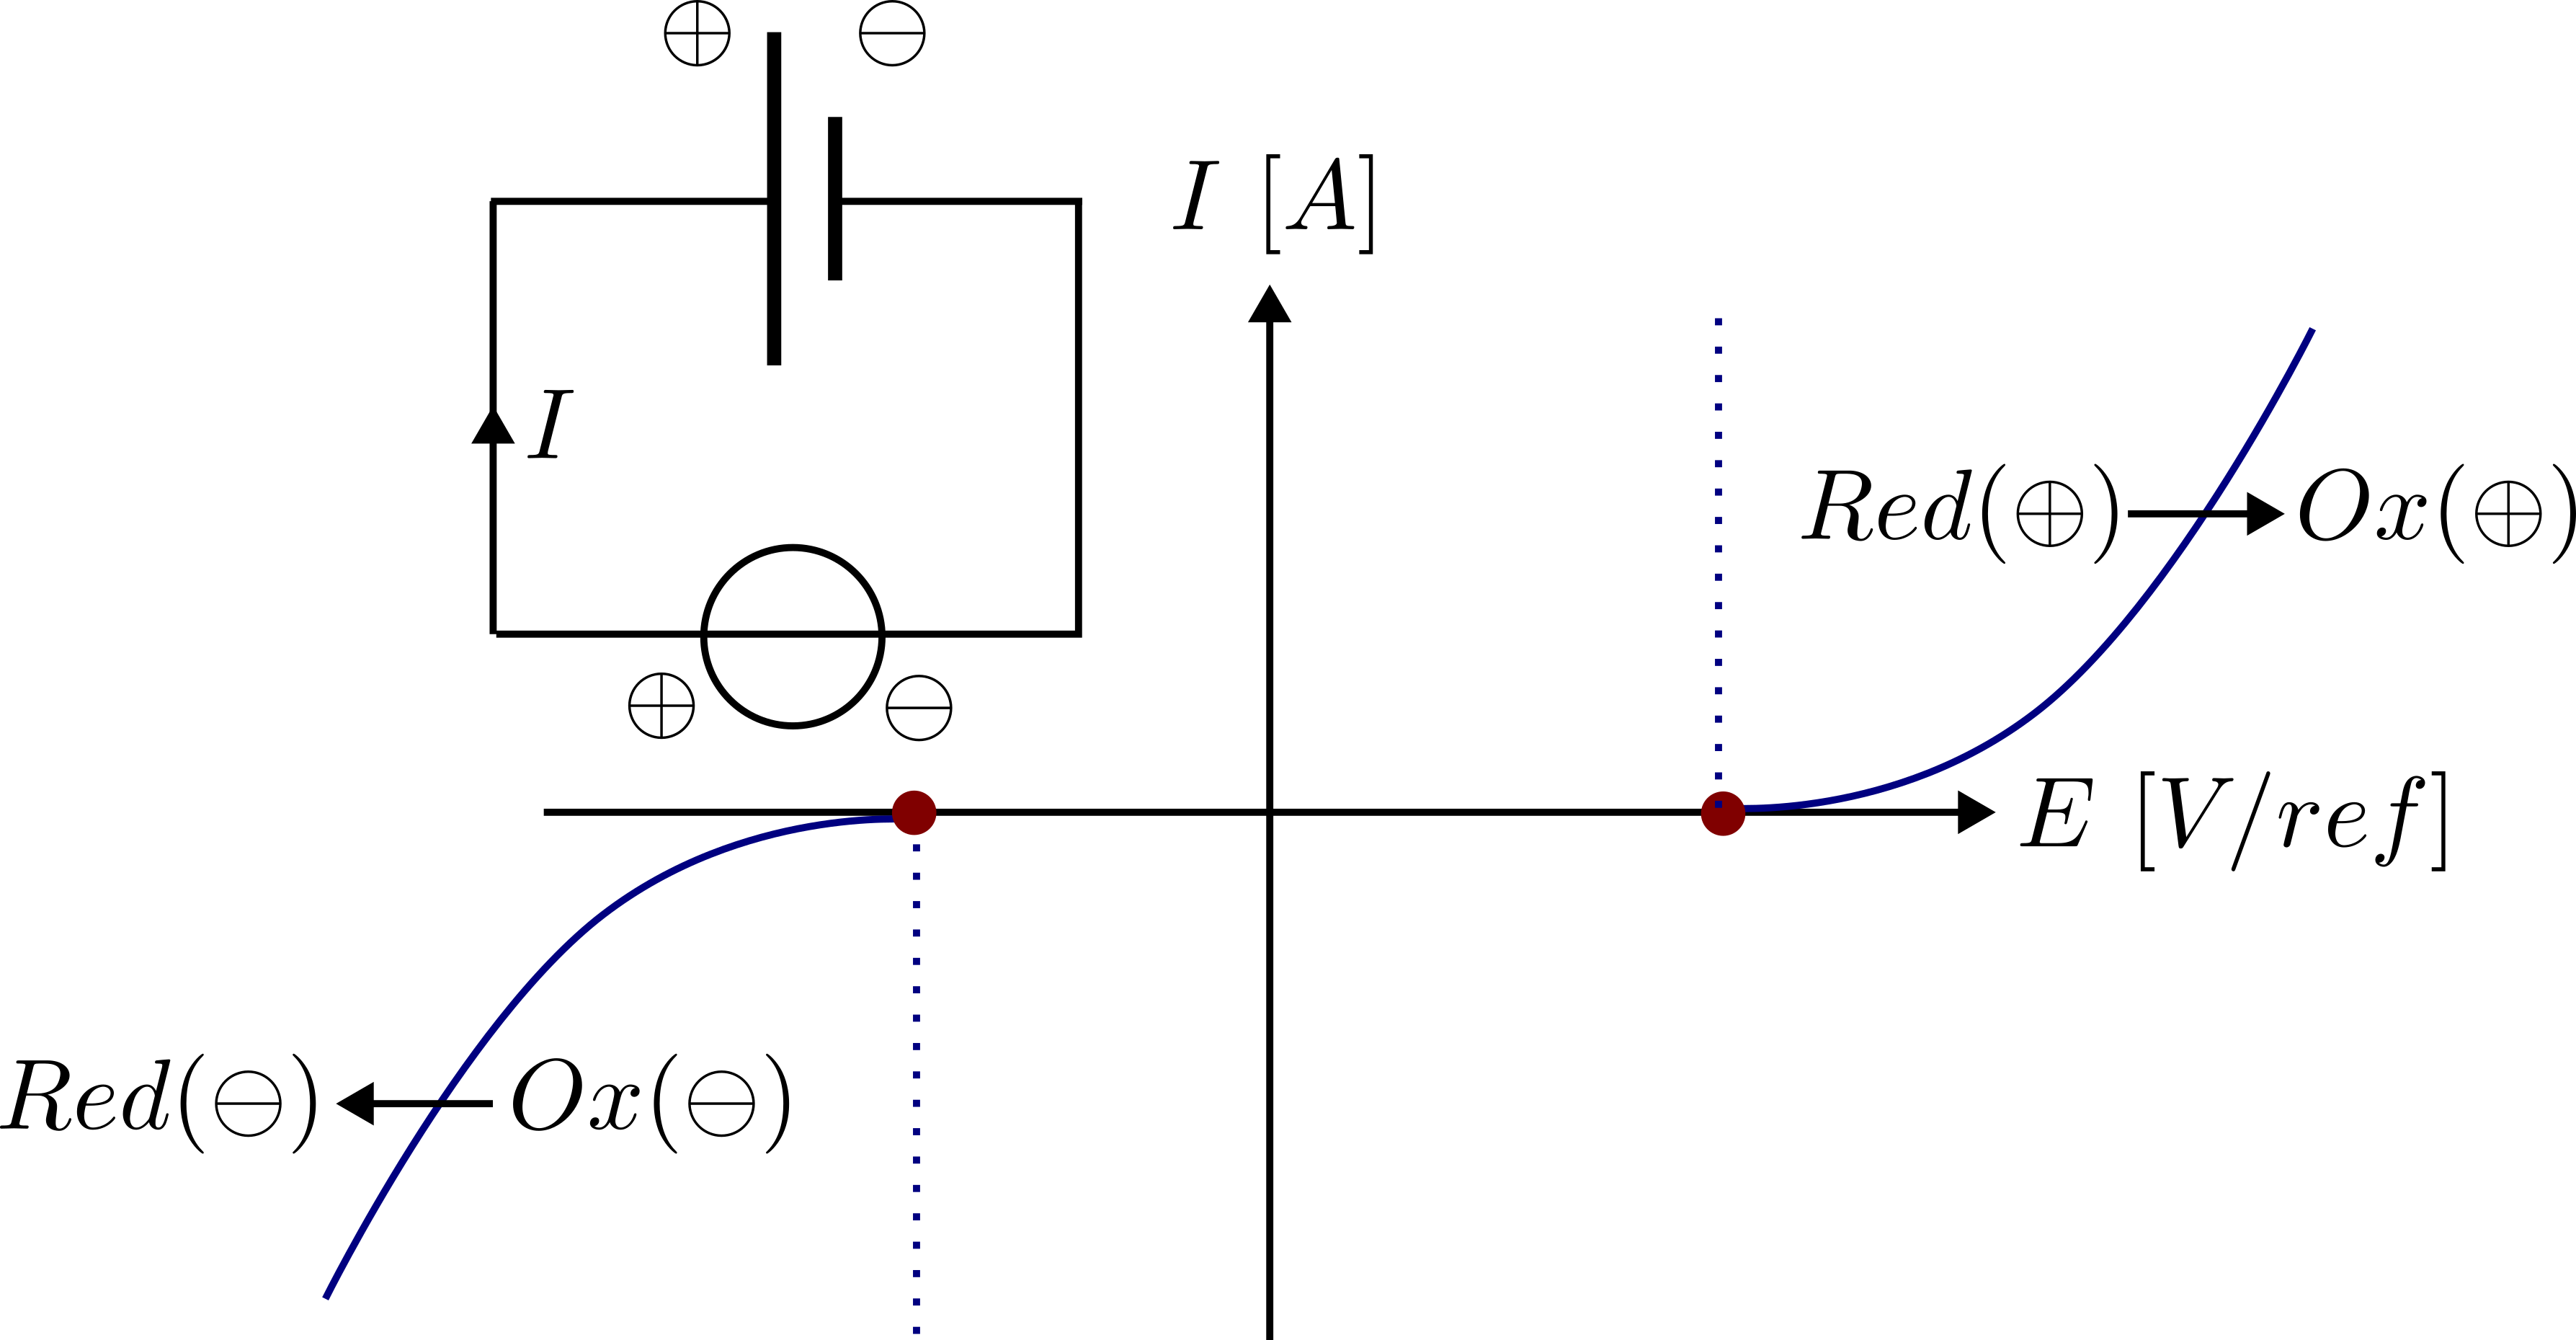
\includegraphics[height=4cm]{figures/Ann03b}}
\end{minipage}\begin{minipage}{0.18\textwidth}
\caption{Courbes courant potentiel montrant l'écart à la thermodynamique dans le cas : \ref{fig:Ann03a} d'une décharge ; \ref{fig:Ann03b} d'une charge}
\end{minipage}
\end{figure}

Si vous avez compris, vous êtes capable d'expliquer à l'enseignant où est-ce qu'on lit la surtension \textbf{anodique} et \textbf{cathodique} de chacun des couples à un courant $I$ donné sur les Fig. \ref{fig:Ann03a} et \ref{fig:Ann03b}. De plus, si vous avez compris ceci, vous pouvez expliquer pourquoi lorsque l'on charge puis décharge un accumulateur à \textbf{courant constant}, le plateau de charge, valeur indiquée par $U_c$, est plus grande que le plateau de décharge, valeur indiquée par $U_d$ :

\begin{figure}[H]
\begin{minipage}{0.68\textwidth}
\centering

\includegraphics[height=5cm]{figures/Ann04}
\end{minipage}\begin{minipage}{0.28\textwidth}
\caption{Allure typique d'une courbe de charge/décharge dans un accumulateur à courant $I$ constant}
\end{minipage}
\end{figure}

Félicitation, vous savez expliquer \textbf{électrochimiquement} le \textbf{phénomène d'hystérèse} observé dans un cycle de charge/décharge (ce point sera réabordé en CM et TD).




\newpage

\section*{Barème}

\begin{minipage}{0.33\textwidth}
Noms-Prénoms du binôme
\end{minipage}\begin{minipage}{0.33\textwidth}
$n^\circ 1$ :
\end{minipage}\begin{minipage}{0.33\textwidth}
$n^\circ 2$ :
\end{minipage}

\begin{questions}
\setcounter{question}{\thefoo}

\titledquestion{Graphes}[1] Qualité des graphes

\titledquestion{Investissement}[2] Variable d'ajustement à la liberté du correcteur en fonction de l'investissement, de la qualité des raisonnements et de la démarche d'investigation du binôme.

\end{questions}

\begin{center}
\gradetable
\bonusgradetable
\end{center}

\end{document}